\chapter{Kinetic inductance detectors: basic theory}
\label{chp:theory}

A KID is a superconducting thin-film microresonator in which the resonator itself is a detector~\autocite{Day2003Nature}.
The detection is performed by using a microwave tone at the KID resonance frequency to measure changes in the electrodynamic response of the film, which is altered by deposited energy.
Figure~\ref{fig:multiplexed_mkids_v1} shows the basic multiplexing concept.
Each detector has a unique resonance frequency, and electronics similar to software-defined radio are able generate and analyze hundreds to thousands of tones simultaneously, allowing many detectors to be multiplexed.

\begin{figure}[htb]
\centering
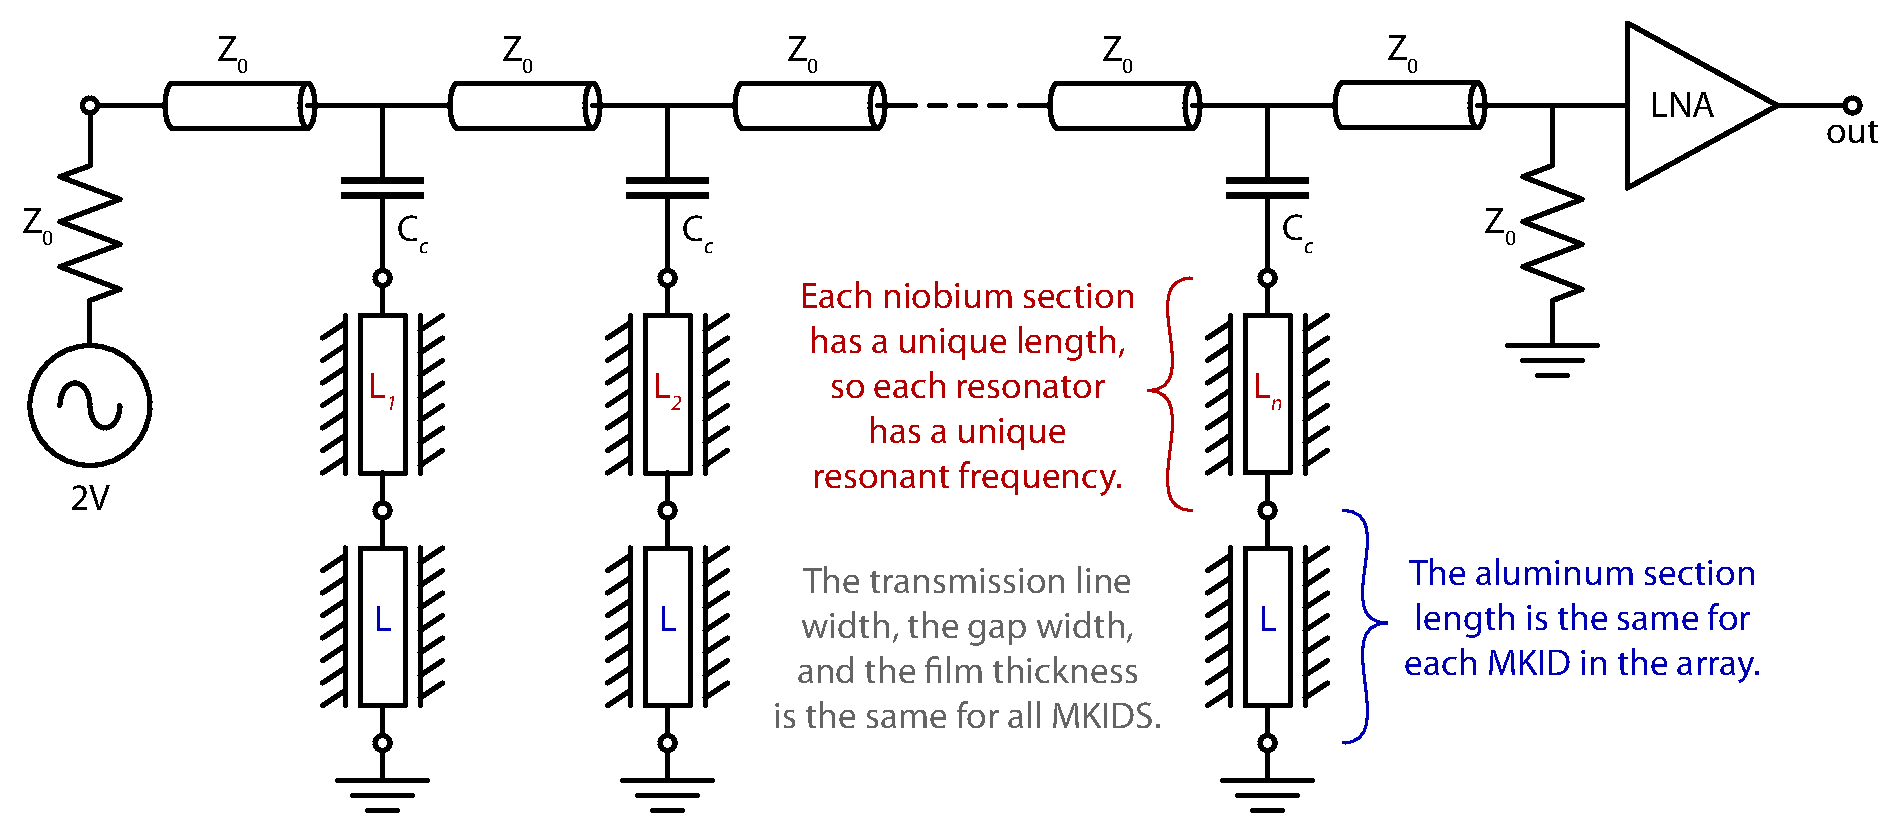
\includegraphics[width=0.8\textwidth]{theory/multiplexed_mkids_v1.pdf}
\caption[A schematic that shows how KIDs are read out and multiplexed.]
{
A schematic that shows how KIDs are read out and multiplexed.
The annotation refers specifically to the KIDs that are discussed in Chapter~\ref{chp:multichroic}, which are made from aluminum and niobium.
The tones are generated at left, propagate past the detectors, and are amplified at right by the low-noise amplifier (LNA).
}
\label{fig:multiplexed_mkids_v1}
\end{figure}

Figure~\ref{fig:introduction_resonator_amplitude_phase} shows how a KID responds to an increase in illumination: the resonance frequency decreases, and the internal dissipation increases.
The changes shown in the plot were due to a change in the temperature of a black body load that illuminated the detectors.

\begin{figure}[htb]
\centering
\includegraphics[width=0.7\textwidth]{theory/introduction_resonator_amplitude_phase.pdf}
\caption[The amplitude and phase of the forward transmission past a resonator, versus frequency.]
{
The amplitude and phase of the forward transmission past a resonator, plotted versus frequency, taken at two different levels of illumination from a beam-filling black body source.
The blue (red) points were taken with the source at \SI{3.3}{K} (\SI{5}{K}).
The small points are the data, the lines are a fit to a resonator model, and the large points mark the resonance frequencies extracted from the fits.
}
\label{fig:introduction_resonator_amplitude_phase}
\end{figure}

In this chapter I introduce the theory that is necessary to understand the response of a KID to light.
Section~\ref{sec:theory.ground_state} contains a quick introduction to the necessary elements of the BCS theory of superconductivity and the superconducting ground state.
In Section~\ref{sec:theory.quasiparticle}, I discuss the generation, scattering, decay, and diffusion of the quasiparticle excitations of a superconductor.
In Section~\ref{sec:theory.electrodynamics}, I discuss superconductor electrodynamics, focusing on the effect of the quasiparticles.
In Section~\ref{sec:theory.perturbation}, I introduce a framework for describing the non-equilibrium state of a superconducting thin film as a small perturbation to the ground state.
In Section~\ref{sec:theory.qpnumber}, I introduce a simplified description of the film in terms of only the total number of quasiparticles, then use this model to motivate and solve the equations that describe the dynamics of the quasiparticle system.
In Section~\ref{sec:theory.resonator}, I discuss a generic model for a shunt-coupled resonator and use it to describe the lumped-element and transmission-line resonators used for the KIDs in this thesis.
In Section~\ref{sec:theory.response}, I use the results from previous sections to derive the response equations for a detector, starting with the absorption of light and ending with the electrical signal that is recorded by the electronics.

\section{The BCS theory and the ground state }
\label{sec:theory.ground_state}

\subsection{The Cooper pair condensate}
\label{sec:theory.ground_state.condensate}

\todo[inline]{Re-read Tinkham and update.}
In the Bardeen-Cooper-Schrieffer (BCS) theory of superconductivity~\autocite{BCS1957PRL, BCS1957PR}, the superconducting ground state can be described in terms of individual-electron (Bloch) states occupied in pairs with opposite momentum and spin, called Cooper pairs~\autocite{Cooper1956PRL}.
These Cooper pairs form due to a phonon-mediated attractive potential $\bcspotential$ between electrons that are within the Debye energy $\phononenergy_\debye$ of the Fermi energy.
The coherence length
$\coherencelength \sim \hbar \velocity_\fermi / \kb \tc$,
where $\velocity_\fermi$ is the Fermi velocity and $\tc$ is the critical temperature for the superconducting phase, corresponds to the minimum size of a Cooper pair as dictated by the uncertainty principle.
For elemental superconductors the coherence length is much greater than the mean spacing between conduction electrons.
While it is more accurate to think of correlations extending over a distance $\coherencelength$, a naive model of the pair condensate is sufficient for the calculations in this thesis.

In a normal metal at temperature $\temperature = 0$, by definition, no states with energy greater than the Fermi energy $\blochenergy_\fermi$ are occupied.
However, in a superconducting metal, even at $\temperature = 0$, some states within an energy range approximately $\kb \tc$ above the Fermi energy remain populated.
The increase in kinetic energy compared to the normal state is outweighed by the decrease in potential energy due to the pairing.

One of the most striking features of the transition to the superconducting state is the Meissner effect, in which, as the temperature is reduced below $\tc$, a screening supercurrent develops to expel any magnetic field from the interior of a bulk superconductor.
This screening is quantified by the penetration depth $\penetrationdepth$, which is the distance from a surface over which the screening supercurrent causes magnetic fields to decay in the bulk.
In the phenomenological London theory, developed long before the BCS theory, the penetration depth at zero temperature is
\begin{equation}
\penetrationdepth_\mathrm{L}
  =
  \left( \frac{\lsvac m_\mathrm{s}}{\impvac n_\mathrm{s} q_\mathrm{s}^2}
  \right)^{1/2},
\end{equation}
where $\lsvac$ is the speed of light in vacuum, $\impvac$ is the impedance of vacuum, and $m_\mathrm{s}$, $n_\mathrm{s}$, and $q_\mathrm{s}$ are respectively the mass, density, and charge of the superconducting carriers.
The aluminum films used for the detectors discussed in this thesis are \SIrange{10}{50}{nm} thick, while the bulk penetration depth for aluminum at low temperature and low frequency is about \SI{50}{nm}~\autocite{Faber1955PRS, Biondi1959bPR}, so the fields completely enter these films. 
The penetration depth is closely related to the reactive part of the superconductor's surface impedance $\impedance_\surface$, discussed in Section~\ref{sec:theory.electrodynamics.surface_impedance} below.

\todo[inline]{Understand time-varying field screening.}
%As in the normal metal, static electric fields are screened over atomic-scale lengths.

In a BCS superconductor below $\tc$, there is a minimum energy $\gap$, called the gap energy, for excitations from the ground state.
These excitations are important for the electrodynamic behavior of a KID, and are discussed in detail later.
In the in the weak-coupling limit of BCS theory, where
$\ssdos \ucvolume \bcspotential \ll 1$,
the critical temperature $\tc$ is proportional to the zero temperature gap energy $\gap_\zerotemp$.
Here, $\ssdos$ is the single spin density of states at the Fermi energy and $\ucvolume$ is the volume of a unit cell.
The relationship is $\gap_\zerotemp = 1.76 \, \kb \tc$, and the numerical factor is accurate to about 20\% in actual elemental superconductors~\autocite{Tinkham2004}.


\subsection{Fiducial parameters}
\label{sec:theory.ground_state.fiducial}

In our current experimental setup we measure the transition temperature either by observing the change in film resistance using a standard four-wire scheme or by observing changes in microwave transmission through the transmission line on a chip containing resonators.
In \SIrange{10}{50}{nm} thick aluminum films we typically measure $\tc$ slightly elevated from the bulk value of \SI{1.2}{K} by \SIrange{0.1}{0.2}{K}, in agreement with other measurements of thin aluminum films~\autocite{Townsend1972PRB}.
Although we are not yet able to directly measure $\gap$, measurements of the gap in thin aluminum films have also shown enhancement above the bulk value~\autocite{Court2008SUST}, and in the absence of a gap measurement we typically assume that the BCS relation remains valid.
Note that some relevant quantities vary exponentially with the ratio of the gap to the temperature, so a small uncertainty in the gap energy may lead to a much larger uncertainty in predictions of such quantities.

As shown in Table~\ref{tab:energies}, the two types of KIDs I discuss here have very different typical resonance frequencies.
In both cases, $\planck \freadout / \gap \ll 1$.
If $\temperature_\bath$ is the bath temperature of the detectors, then for the single-polarization lumped-element KIDs $\planck \freadout_\singlepol / \kb \temperature_\bath \ll 1$, while for the multichroic co-planar waveguide KIDs $\planck \freadout_\multichroic / \kb \temperature_\bath \approx 1$.
This distinction is not practically important for the readout photon occupancy, because the readout power is always sufficiently high to produce an occupancy much greater than one.

\begin{table}[htb]
\centering
\caption
[Fiducial energies, temperatures, and frequencies.]
{
Fiducial energies, temperatures, and frequencies:
$\tc$ is close to the critical temperature we typically measure in aluminum films;
$\temperature_\bath$ is a typical bath temperature; 
$\freadout_\singlepol$ is a typical resonance frequency for the single-polarization lumped-element KIDs used in experiments discussed in Chapters~\ref{chp:loss}~and~\ref{chp:sensitivity};
$\freadout_\multichroic$ is a typical resonance frequency for the multichroic CPW KIDs discussed in Chapter~\ref{chp:multichroic}.
I use these values for numerical estimates, including the slightly elevated gap and critical temperature.
}
\renewcommand{\arraystretch}{1.2}
\begin{tabular}{c S S S S}
\toprule
Parameter & \si{J} & \si{\micro eV} & \si{GHz} & \si{K} \\
\midrule
$\gap_\zerotemp$ & 3.16e-23 & 197.16 & 47.67 & 2.288 \\
$\tc$ & 1.79e-23 & 112.03 & 27.09 & 1.300 \\
$\freadout_\multichroic$ & 1.99e-24 & 12.41 & 3.00 & 0.144 \\
$\temperature_\bath$ & 1.79e-24 & 11.20 & 2.71 & 0.130 \\
$\freadout_\singlepol$ & 6.63e-26 & 0.41 & 0.10 & 0.005 \\
\bottomrule
\end{tabular}
\label{tab:energies}
\end{table}

KIDs have been made from numerous materials, some of which are not well-described by the BCS theory.
However, the KIDs discussed in this work are made either from only aluminum or from both aluminum and niobium, both of which are BCS superconductors.
Throughout this thesis, when making numerical estimates, I use typical material parameters for aluminum and niobium given in Table~\ref{tab:materials} along with the fiducial values given in Table~\ref{tab:energies}, including the slightly elevated values of $\tc$ and $\gap$ that we typically measure.
These should give reasonable descriptions of the detectors we have tested.

\todo[inline]{Check N0 for niobium and understand values given by Kaplan et al.}
\begin{table}[htb]
\centering
\caption[Parameters of superconducting metals used in this thesis.]
{
Parameters of superconducting metals used in this thesis.
See Table~\ref{tab:notation.condensed_matter} for the symbol definitions.
Values are from \textcite{Kaplan1976PRB} except where noted.
}
\renewcommand{\arraystretch}{1.2}
\begin{tabular}{c c c c}
\toprule
Parameter & Unit & Aluminum & Niobium \\
\midrule
$\tc$ (bulk) & \si{K} & 1.19 & 9.2 \\
%$\gap_\zerotemp$ & {} & {} & {} \\ 
$\ssdos$ & \si{eV^{-1}.\micro\meter^{-3}} & \num{1.74e10}~\autocite{Thomas2015SUST} & \num{8.52e10}~\autocite{Jani1988PRB} \\
$\electronphonontime$ & \si{ns} & 438 & 0.149 \\
\bottomrule
\end{tabular}
\label{tab:materials}
\end{table}

\subsection{Radiation detection using superconductors}
\label{sec:theory.ground_state.detection}

For a KID absorbing pair-breaking radiation, the cutoff (lowest detectable) frequency is
\begin{equation}
\foptical_\cutoff 
  =
  2 \gap / \planck
  \approx
  3.5 \, \kb \tc / \planck
  \approx
  \SI{74}{GHz} \left( \tc / \SI{1}{K} \right).
\end{equation}
To minimize the rate of thermal excitations, KIDs must be operated at a low bath temperature.
If $\temperature_\bath$ is the practically achievable bath temperature for a large detector array designed to detect photons with frequency $\foptical$, the superconducting energy gap must satisfy
\begin{equation}
\planck \foptical / 2
  >
  \gap
  \gg
  \kb \temperature_\bath.
\end{equation}
Fortunately, this is currently possible over at least part of the frequency range relevant for CMB observations.
Aluminum can be used to detect pair-breaking photons with frequencies above
$\foptical_\cutoff \approx \SI{100}{GHz}$.
Refrigeration using adiabatic demagnetization or helium dilution allows for cooling of large arrays to temperatures
$\temperature_\bath \approx \SI{0.1}{K} \sim \tc / 10$,
sufficiently low that thermal excitations are negligible.
This allows KIDs to achieve, in principle, the fundamental sensitivity limit set by the statistics of photon arrival.

\section{Quasiparticle excitations}
\label{sec:theory.quasiparticle}

\subsection{The quasiparticle density of states}
\label{sec:theory.quasiparticle.dos}

The quasiparticle excitations that are orthogonal to the ground state are neither lone electron nor hole excitations, but are superpositions of excitations on both sides of the Fermi surface.
These excitations are commonly called Bogoliubov quasiparticles, and I refer to them simply as quasiparticles.
They have spin $1 / 2$ and thus obey Fermi statistics.
Their canonical decay mechanism is to rejoin the condensate by recombining in pairs to form a Cooper pair and emitting a phonon.
Other decay channels are discussed below.

Because of the gap, there are no low-energy states into which the constituents of the Cooper pairs can individually scatter, and a supercurrent can thus flow with no resistance, at least at zero frequency.
However, like the conduction electrons of the normal metal, the quasiparticles experience lossy scattering.
Thus, the conductivity at nonzero frequencies, while typically much higher than in even an excellent normal conductor, is finite.
A KID detects radiation essentially by measuring these excitations through their effect on the surface impedance of the superconductor at microwave frequencies.

\todo[inline]{update after reading AM}
The energy of a Bloch state with wavevector $\vwvec$ is
$\blochenergy_{\vwvec} = \hbar^2 \wvec^2 / 2 \mass$
for an electron mass $\mass$.
If $\blochenergyf_{\vwvec} = \blochenergy_{\vwvec} - \blochenergy_\fermi$ is the same energy relative to the Fermi energy $\blochenergy_\fermi$, then the energy of a quasiparticle with wavevector $\vwvec$ is
\begin{equation}
\energy_{\vwvec}
  =
  \left( \blochenergyf_{\vwvec}^2 + \gap^2 \right)^{1/2},
\label{eqn:qpenergy}
\end{equation}
which is positive for excitations on both the ``electron'' branch outside the Fermi surface, with $\blochenergyf > 0$, and the ``hole'' branch inside the Fermi surface, with $\blochenergyf < 0$.
This relationship between the Bloch state energy and the quasiparticle energy is plotted in Figure~\ref{fig:quasiparticle_energy_and_density_of_states}(a).

\todo[inline]{Recreate BCS figure.}
\begin{figure}[htb]
\centering
\includegraphics[width=\textwidth]{theory/quasiparticle_energy_and_density_of_states.pdf}
\caption
[The quasiparticle energy and density of states.]
{
\textbf{(a)}
The BCS quasiparticle energy $\energy$ versus the Bloch state energy $\blochenergyf$ in units of the gap.
Here, the Fermi energy is at $\blochenergyf = 0$.
\textbf{(b)}
The reduced density of states $\qprdos$ versus the quasiparticle energy $\energy$ in units of the gap.
For display, the three density of states curves have all been broadened by adding small imaginary parts to the gap:
$\gap \rightarrow \gap - \I \mitrovic$.
The gray horizontal line shows $\qprdos = 1$, which is the asymptotic value at high $\energy$.
%(If the corresponding energies were plotted in (a), they would have very narrow dips near $\blochenergyf = 0$ down to a minimum near $\energy / \gap = 0$.)
}
\label{fig:quasiparticle_energy_and_density_of_states}
\end{figure}

The range of energies involved forming the superconducting state is small compared to the Fermi energy.
Because the normal metal density of states does not change much over this range of energies, it is conventional to take it to be constant and to define $\ssdos$ to be the number of electron states of one spin per unit energy per unit volume at the Fermi energy.
The BCS density of states arises from the relationship between the quasiparticle energy $\energy$ and the Bloch energy $\blochenergyf$:
\begin{equation}
\dd{\energy}
  =
  \dd{\left( \blochenergyf^2 + \gap^2 \right)^{1/2}}
  =
  \frac{\blochenergyf \dd{\blochenergyf}}{\left( \blochenergyf^2 + \gap^2 \right)^{1/2}},
\end{equation}
so
\begin{equation}
\dd{\blochenergyf}
  =
  \frac{\energy \dd{\energy}}{\left(\energy^2 - \gap^2 \right)^{1/2}}.
\end{equation}
The density of quasiparticle states is thus
\begin{equation}
\supssdos(\energy)
  =
  \ssdos \dv{\blochenergyf}{\energy}
  =
  \ssdos \frac{\energy}{(\energy^2 - \gap^2)^{1/2}}
  \equiv
  \ssdos \qprdos(\energy),
\label{eqn:supssdos}
\end{equation}
where $\qprdos$ is the \textit{normalized} (or \textit{reduced}) density of states.
There is a one-to-one correspondence between the Bloch states and the quasiparticle states, so the total number of states is the same as for the normal metal.
The quasiparticle density of states versus quasiparticle energy is plotted in Figure~\ref{fig:quasiparticle_energy_and_density_of_states}(b).

While the BCS density of states has a singularity at $\energy = \gap$, in an actual superconductor this singularity will be smeared out at least slightly.
A supercurrent, always present in an operating KID due to the readout tone, causes some broadening of the density of states~\autocite{Anthore2003PRL}, as may granularity~\autocite{Dynes1984PRL}, disorder~\autocite{Driessen2012PRL}, and impurities~\autocite{ONeil2008PRL, ONeil2010JAP} in the film.
Such broadening of the density of states is often modeled, at least for energies near the gap, by writing the BCS reduced density of states as
\begin{equation}
\qprdos(\energy)
  =
  \Re{\frac{\energy}{(\energy^2 - \gap^2)^{1/2}}}
\end{equation}
and introducing a small imaginary part to either the quasiparticle energy
$\energy \rightarrow \energy - \I \dynes$~\autocite{Dynes1984PRL}
or the gap energy
$\gap \rightarrow \gap - \I \mitrovic$~\autocite{Mitrovic2008JPCM}.
Figure~\ref{fig:quasiparticle_energy_and_density_of_states}(b) shows density-of-states curves calculated using the latter procedure.
Both of these expressions describe a nonzero density of states for energies $\energy < \gap$.
The density of states may be measured in tunneling experiments, for example, but since we have not performed such experiments I will assume it changes little from the BCS form.
Although the density of states may be identically zero below some energy $\energy_\mathrm{min}$, with $\gap \ge \energy_\mathrm{min} > 0$, I will allow for the possibility of sub-gap states by writing integrals over quasiparticle energy with their lower limit set to 0, taking the cutoff to be present in the density of states.

In superconductor out of thermal equilibrium, the quasiparticle occupancy may differ between pairs of wavevectors on either side of the Fermi surface that correspond to quasiparticle states with the same energy, and may also differ between two spin states with the same wavevector.
Fortunately, we can ignore these distinctions.
The relevant quasiparticle excitation mechanisms, namely photons and phonons, populate both branches and both spin states equally on average~\autocite{Tinkham2004}.
In the absence of spin injection and external magnetic fields, we do not expect significant splitting of the density of states for opposite spin directions~\autocite{Meservey1970PRL}.
Thus, we can adequately describe the quasiparticle system using an occupancy function $\qpoccupancy(\energy)$ that has the same dependence on the quasiparticle energy for both branches and for both spin directions.
In thermal equilibrium at temperature $\temperature$, the occupancy is 
$\qpoccupancy(\energy, \temperature) = [\exp(\energy / \kb \temperature) + 1]^{-1}$,
the Fermi-Dirac function.
However, KIDs are typically operated out of equilibrium.

The quasiparticle density for an arbitrary $\qpoccupancy(\energy)$ is
\begin{equation}
\qpdensity
  =
  4 \ssdos
  \int_{0}^{\infty} \dd{\energy}
  \qprdos(\energy) \qpoccupancy(\energy),
\label{eqn:qpdensity}
\end{equation}
where one factor of two comes from the branches on either side of the Fermi energy, and the other comes from a sum over spins.
At low temperatures the gap will be close to its zero-temperature value $\gap_\zerotemp$, and the Fermi-Dirac occupancy is approximately
$\qpoccupancy(\energy) \approx \exp (-\energy / \kb \temperature)$.
Then, as derived in Appendix~\ref{chp:first-order_response}, the quasiparticle density is
\begin{equation}
\qpdensity(\temperature)
  =
  4 \ssdos \gap_\zerotemp
  K_1(\gap_\zerotemp / \kb \temperature)
  \approx
  4 \ssdos \gap_\zerotemp
  \left( \frac{\pi \kb \temperature}{2 \gap_\zerotemp} \right)^{1/2}
  \exp \left( -\frac{\gap_\zerotemp}{\kb \temperature} \right),
\label{eqn:qpdensity_thermal}
\end{equation}
where $K_1$ is the first-order modified Bessel function of the second kind.
These approximate expressions are plotted in Figure~\ref{fig:reduced_thermal_qpdensity}.
\todo[inline]{Recreate $\qpdensity$ figure and compare to exact BCS expression.}
The quantity $\ssdos \gap_\zerotemp$ frequently appears (usually with a prefactor of 2 or 4) as a characteristic quasiparticle density.
For aluminum,
$\ssdos \gap_\zerotemp \approx \SI{3.4e6}{\micro\meter^{-3}}$,
which is much larger than a typical operating density.
The quasiparticle density is discussed in more detail in Section~\ref{sec:theory.qpnumber}, where it replaces the occupancy as the quantity used to describe the quasiparticle system.

\begin{figure}[htb]
\centering
\includegraphics[width=\textwidth]{theory/reduced_thermal_qpdensity.pdf}
\caption
[The reduced thermal quasiparticle density versus reduced temperature.]
{The reduced thermal quasiparticle density versus reduced temperature, from Equation~\ref{eqn:qpdensity_thermal}.
The gap $\gap$ here is taken to be equal to its value at $\temperature = 0$, which at higher temperatures is not a good approximation.}
\label{fig:reduced_thermal_qpdensity}
\end{figure}

The quasiparticles affect the gap energy, which decreases as the quasiparticle density increases.
The BCS theory gives an implicit equation for the gap:
\begin{equation}
1
  =
  \ssdos \ucvolume \bcspotential
  \int_\gap^\infty \dd{\energy}
  \qprdos(\energy) \frac{1 - 2 \qpoccupancy(\energy)}{\energy},
\end{equation}
where the gap appears in both the lower limit of the integral and in the quasiparticle energy.
(The unit cell volume appears here because I use $\ssdos$ to mean the number of single-spin normal-metal states per unit energy \textit{per unit volume} at the Fermi energy.)
In Section~\ref{sec:theory.perturbation} I discuss a method for obtaining approximate equations for the gap.
Even in an illuminated KID, the number of excitations will generally be sufficiently small that the gap will not vary much from its value at zero temperature.


\subsection{Generation}
\label{sec:theory.quasiparticle.generation}

The quasiparticle excitations must occur in pairs, since the energy reduction is due to the pairing, so a particle that deposits energy greater than $2 \gap$ (the \textit{spectroscopic} gap) can break one or more Cooper pairs, exciting quasiparticles that eventually recombine into Cooper pairs or decay by other means.
Phonons with energy $\phononenergy > 2 \gap$ that enter the film from the substrate may also break pairs.

As we will see later, the detector sensitivity may be increased by using a high readout tone power.
Although the readout photons individually have energies much less than the gap (see Table~\ref{tab:energies}), a quasiparticle that absorbs many quanta and is excited to an energy above $3 \gap$ may scatter inelastically and create a phonon that is sufficiently energetic to break a pair.
KID experiments that use careful shielding to reduce quasiparticle generation due to stray light nevertheless observe more quasiparticles than the thermal equilibrium value, and some of this excess is typically attributed to readout generation~\autocite{deVisser2012APL,deVisser2014NatComm}.


\subsection{Pair recombination}
\label{sec:theory.quasiparticle.pair_recombination}

Quasiparticles have finite lifetimes and may decay in various ways.
For elemental BCS superconductors, the most relevant process involves two quasiparticles with energies
$\energy_1, \energy_2 \ge \gap$
recombining into a Cooper pair with the emission of a phonon with energy
$\phononenergy = \energy_1 + \energy_2 \ge 2 \gap$.
(Since a photon can break a Cooper pair and excite quasiparticles, the reverse process of recombination with photon emission is possible.
However, because the final density of states corresponding to this process is much smaller than the density of states for phonon emission, the radiative lifetime is much longer and this process is negligible~\cite{Burstein1961PRL}.)
\todo[inline]{Incorporate other refs in Rothwarf and Taylor}

\textcite{Kaplan1976PRB} derive a low-temperature equilibrium pair-recombination time, given for a quasiparticle with $\energy = \gap_\zerotemp$ by
\begin{equation}
\qprecombinationtime^{-1}
  =
  \electronphonontime^{-1}
  \pi^{1/2}
  \left( \frac{2 \gap_\zerotemp}{\kb \tc} \right)^{5/2}
  \left( \frac{\temperature}{\tc} \right)^{1/2}
  \exp \left( -\frac{\gap_\zerotemp}{\kb \temperature} \right),
\label{eqn:qprecombinationtime}
\end{equation}
where $\electronphonontime$ is the characteristic electron-phonon interaction time defined in the same reference.
The recombination rate for a given total energy is proportional to the phonon density of states at that energy, which increases with increasing energy~\autocite{Chang1978JLTP}.
Thus, quasiparticles with higher energies have shorter lifetimes.
Comparing Equation~\ref{eqn:qprecombinationtime} to Equation~\ref{eqn:qpdensity_thermal} shows that, in thermal equilibrium, the inverse recombination lifetime is proportional to the quasiparticle density:
\begin{equation}
\qprecombinationtime^{-1}
  =
  \electronphonontime^{-1}
  \left( \frac{2 \gap_\zerotemp}{\kb \tc} \right)^3
  \frac{\qpdensity}{4 \ssdos \gap_\zerotemp}.
\end{equation}
The proportionality
\begin{equation}
\qprecombination
  \equiv
  \left( \frac{2 \gap_\zerotemp}{\kb \tc} \right)^3
  \left( 4 \ssdos \gap_\zerotemp \electronphonontime \right)^{-1}
\label{eqn:qprecombination}
\end{equation}
is the quasiparticle recombination constant~\autocite{Gray1981Chapter5}.
Using values for aluminum from Table~\ref{tab:materials} gives
$\qprecombination = \SI{7.8}{\micro\meter^3.\second^{-1}}$.
The recombination constant will actually change as the gap energy varies with quasiparticle density~\autocite{Gray1971JPF, Rothwarf1974PRL}, but I will neglect this dependence.
The recombination rate per unit volume is thus quadratic in the quasiparticle density:
\begin{equation}
\rate_\qprecombination
  \equiv
  \qprecombinationtime^{-1} \qpdensity
  =
  \qprecombination \qpdensity^2.
\label{eqn:rate_qprecombination}
\end{equation}
Since recombination involves quasiparticles interacting in pairs, it is not surprising that the rate for $\qpnumber$ quasiparticles goes as $\binom{\qpnumber}{2} \propto \qpnumber^2$ to leading order~\autocite{Gray1971JPF}.

In thermal equilibrium, if quasiparticles are generated at a rate $\rate_\generation(\temperature)$ per unit volume and the only quasiparticle decay process is recombination with phonon emission, then the rate equation for the quasiparticle density is
\begin{equation}
0
  =
  \dv{\qpdensity}{\time}
  =
  \rate_{\generation}(\temperature)
  -
  \qprecombination \qpdensity(\temperature)^2.
\label{eqn:rate_qpdensity_thermal}
\end{equation}
Then, using Equation~\ref{eqn:qpdensity_thermal}, the low-temperature thermal generation rate is
\begin{equation}
\rate_{\generation}(\temperature)
  =
  \frac{4 \ssdos \gap_\zerotemp}{\electronphonontime} \left( \frac{2 \gap_\zerotemp}{\kb \tc} \right)^3 K_1(\gap_\zerotemp / \kb \temperature)^2
  \approx 
  \frac{4 \ssdos \gap_\zerotemp}{\electronphonontime} \left( \frac{2 \gap_\zerotemp}{\kb \tc} \right)^3 \frac{\pi \kb \temperature}{2 \gap_\zerotemp} \exp \left(-\frac{2 \gap_\zerotemp}{\kb \temperature}\right).
\label{eqn:rate_generation_thermal}
\end{equation}
At sufficiently low temperatures the total thermal generation rate will become negligible compared to other sources.
This reduces the effect of fluctuations in the generation rate cause by temperature fluctuations, which are common in a moving telescope.


\subsection{Phonons}
\label{sec:theory.quasiparticle.phonons}

While the various generation process act to create an occupancy that exceeds the thermal value, scattering processes act to restore the quasiparticle system to equilibrium.
\textcite{Kaplan1976PRB} derive a thermal equilibrium quasiparticle-phonon scattering time given by
\begin{equation}
\qpphononscatteringtime^{-1}
  =
  \electronphonontime^{-1} \Gamma \left(\tfrac{7}{2}\right) \zeta \left(\tfrac{7}{2}\right) \left( \frac{\kb \tc}{2 \gap_\zerotemp} \right)^{1/2} \left( \frac{\temperature}{\tc} \right)^{7/2},
\label{eqn:electron-phonon_scattering}
\end{equation}
where $\Gamma$ is the Gamma function and $\zeta$ is the Riemann zeta function.
Assuming the BCS weak-coupling relation, the numerical factors work out to
$\Gamma (7 / 2) \zeta (7 / 2) / 3.52^{1/2} \approx 1.996$.
\todo[inline]{Give scattering time with fiducial parameters.}
A quasiparticle at the gap edge cannot scatter and emit a phonon, because there no available quasiparticle states with lower energy, but at higher energies the scattering rate rapidly increases.
\todo[inline]{What about impurity scattering?}
\todo[inline]{What is the effect of electron-electron scattering? Allegedly important for aluminum. See ChangJLTP1978.}

A phonon produced by quasiparticle recombination has sufficient energy to break another Cooper pair in the same superconductor.
Such a phonon will quickly encounter the film-substrate interface, but the acoustic match between superconducting films and typical crystalline substrates tends to be poor, so phonons are likely to reflect on each encounter with the  interface~\autocite{Kaplan1979JLTP}.
These facts will significantly modify the results of the preceding section.

%In aluminum, \textcite{Kaplan1976PRB} calculate an average time $\phononpairbreakingtime = \SI{242}{ps}$ for a sufficiently energetic phonon to break a Cooper pair at low temperature, and the time decreases with increasing phonon energy.
\textcite{Chang1978JLTP} calculate a time
$\phononpairbreakingtime \sim \SI{100}{ps}$
for a sufficiently energetic phonon to break a pair, which is much less than both the inelastic scattering time and the anharmonic decay time~\autocite{Kozorezov2000PRB}.
They also calculate a phonon escape time
\begin{equation}
\phononescapetime
  =
  \frac{4 \thickness}{\efficiency \soundspeed},
\label{eqn:phononescapetime}
\end{equation}
where $\thickness$ is the film thickness, $\soundspeed$ is the speed of sound, and $\efficiency$ is the transmission probability per encounter, which may be quite small~\autocite{Kaplan1979JLTP}.
Using
$\thickness = \SI{40}{nm}$
and
$\soundspeed = \SI{6.4e3}{m.s^{-1}}$~\autocite{Chang1978JLTP}
gives
$\phononescapetime = \SI{25}{ps} / \efficiency$.

A recombination phonon must leave the film for the quasiparticle number to decrease, so the effective recombination lifetime of the quasiparticles is increased by a phonon-trapping factor~\autocite{Rothwarf1967PRL}
\begin{equation}
\phonontrapping
  =
  \left( \frac{\phononescapetime^{-1}}{\phononescapetime^{-1} + \phononpairbreakingtime^{-1}} \right)^{-1}
  =
  1 + \frac{\phononescapetime}{\phononpairbreakingtime},
\label{eqn:phonontrapping}
\end{equation}
where $\phonontrapping^{-1}$ is the probability for a phonon to escape the film instead of breaking a pair.
Depending on the composition and thickness of the film and substrate, and the details of their interface, this probability may range from just above 0 to just less than 1.
Since both the pair-breaking and escape times are much less than the quasiparticle recombination time $\qprecombinationtime$, which is usually \SIrange{1}{1000}{\micro\second} in the superconductors used for KIDs, the time spent as a phonon is negligible and nearly all of the energy resides in the quasiparticles~\autocite{Rothwarf1974PRL}.
Phonons, produced by scattering or otherwise, for which $\phononenergy < 2 \gap$ are subject to the same phonon trapping effect, but this is less important because these phonons cannot break pairs.

To capture the relevant effects of phonon trapping, we may replace the recombination constant $\qprecombination$ by an effective recombination constant
$\qprecombinationeff = \qprecombination / \phonontrapping$
in Equations~\ref{eqn:rate_qprecombination} and~\ref{eqn:rate_qpdensity_thermal}.
(Note that the thermal density of quasiparticles is independent of $\phonontrapping$: the effective quasiparticle recombination lifetime is increased by a factor $\phonontrapping$, but the thermal generation rate due to pair-breaking thermal phonons entering from the substrate is decreased by the same factor.)
Because $\phonontrapping$ is material-dependent and difficult to calculate~\autocite{Gray1981Chapter5}, the fundamental quasiparticle recombination time $\qprecombinationtime$, and thus the characteristic electron-phonon time $\electronphonontime$, are not experimentally accessible from measurements of KIDs.

\todo[inline]{Incorporate material on thickness-independent trapping}
\begin{comment}
According to Equation~\ref{eqn:phononescapetime}, the phonon trapping factor should decrease with decreasing film thickness.
\textcite{Eisenmenger1976AP}, using a ballistic phonon model and assuming specular reflection at interfaces, point out that when the film thickness $\thickness$ is much less than the mean-free path against pair-breaking, the escape time is independent of the film thickness and depends only on the critical angle for total internal reflection.
However, there seems to be no experimental evidence for this regime.
Measurements of the phonon trapping factor in aluminum films as thin as \SI{100}{nm} have shown linear dependence on film thickness [cite Long].
\end{comment}

\todo[inline]{Incorporate material on qp-phonon imbalance at short times}
%the imbalance between quasiparticles and phonons at times $\time \ll \qprecombinationtime$~\autocite{Rothwarf1967PRL}.

This model ignores the phonon population in the substrate.
The anharmonic decay time is very long in silicon~\autocite{Maris1993PRB}, so phonons that do escape from the film cannot necessarily be neglected unless they are efficiently destroyed.
\textcite{deVisser2014} shows data (in Appendix B) consistent with a large population of recombination phonons in the substrate forming the bottleneck for relaxation of the quasiparticle system.
\textcite{Patel2017PRB} show that pair-breaking phonons can propagate for several millimeters across a chip, and that they are absorbed by normal metal regions.
Phonons that escape from one detector and are absorbed in another could cause spurious response, an effect called crosstalk.


\subsection{Single-quasiparticle decay}
\label{sec:theory.quasiparticle.single_decay}

In addition to canonical recombination in pairs with phonon emission, quasiparticles may also decay through processes that decrease their number by 1.
For these processes, the total decay rate per unit volume is proportional to the quasiparticle density.

For example, magnetic flux vortices act as quasiparticle sinks~\autocite{Ullom1998APL,Wang2014NatComm}.
The gap energy is reduced inside a vortex, so a quasiparticle that diffuses into one may scatter inelastically to an energy below the gap energy outside.
It will thus remain trapped inside the vortex, and when it eventually recombines with another quasiparticle the resulting phonon energy may be less than $2 \gap$, insufficient to break a pair outside the vortex.
Quasiparticles may also become trapped in local defects~\autocite{Kozorezov2001APL} or in normal metal regions in contact with the superconductor~\autocite{Joyez1994PRL, Riwar2016PRB}.

The decay rate per unit volume due to all such single-quasiparticle sources can be written
\begin{equation}
\rate_\qpsingledecay
  =
  \sum_\alpha \qpsingledecay_\alpha \qpdensity
  \equiv
  \qpsingledecay \qpdensity,
\label{eqn:rate_qpsingledecay}
\end{equation}
where $\qpsingledecay$ is the sum of the decay constants for the individual processes.
These processes may be useful for detector engineering, but they  are not necessary to describe most of the behavior of the KIDs discussed in this work.


\subsection{Inhomogeneity and diffusion}
\label{sec:theory.quasiparticle.inhomogeneity}

While the quasiparticles are collective excitations of electrons near the Fermi surface, their typical velocities are much less than the Fermi velocity $\velocity_\fermi$.
In fact, the velocity of a quasiparticle with $\energy = \gap$ is zero.
The BCS relationship between quasiparticle group velocity $\velocity_\group$ and quasiparticle energy $\energy$ is
\begin{align}
\velocity_\group
  =
  \pdv{\energy_\momentum}{\momentum}
  =
  \frac{\blochenergyf_\momentum}{\energy_\momentum} \frac{\momentum}{\mass},
\end{align}
where $\momentum$ and $\mass$ are the electron momentum and mass.
The energy range where the quasiparticle occupancy is nonzero is a small fraction of the Fermi energy, so we take
$\momentum / \mass = \velocity_\fermi$.
Then,
\begin{equation}
\velocity_\group(\energy)
  =
  \velocity_\fermi \left( 1 - \frac{\gap^2}{\energy^2} \right)^{1/2}.
\end{equation}
As shown in Figure~\ref{fig:quasiparticle_group_velocity}, the group velocity rapidly increases with increasing quasiparticle energy to a significant fraction of the Fermi velocity.

\begin{figure}[htb]
\centering
\includegraphics[width=0.9\textwidth]{theory/quasiparticle_group_velocity.pdf}
\caption[The quasiparticle group velocity versus quasiparticle energy.]
{
The quasiparticle group velocity normalized to the Fermi velocity versus quasiparticle energy normalized to the gap energy.
The blue curve is universal.
The vertical lines correspond to the energy of the gap plus one readout photon for the two fiducial readout frequencies, assuming the fiducial value for the gap energy.
We expect the first peaks in the occupancy to occur at these energies.
}
\label{fig:quasiparticle_group_velocity}
\end{figure}

The quasiparticle diffusion coefficient $\qpdiffusion$ is related to the normal-state diffusion coefficient $\normaldiffusion$ by
\begin{equation}
\qpdiffusion
  =
  \frac{\expval{\velocity_\group}}{\velocity_\fermi} \normaldiffusion,
\end{equation}
where $\expval{\velocity_\group}$ is the group velocity averaged over all quasiparticles~\autocite{Ullom1998PRB}.
The rapid variation of the group velocity with energy makes it difficult to estimate the quasiparticle diffusion coefficient without a good estimate of the nonequilibrium occupancy.
Assuming only pair recombination is relevant, a typical diffusion distance is then
$(\qpdiffusion \phonontrapping \qprecombinationtime)^{1/2}$.
This is usually long enough to reduce the problem to two dimensions.
\todo[inline]{Calculate fiducial diffusion length!}

With $\qpdensity(\time, \vb{x})$ the position-dependent density and $\nabla^2$ the Laplacian, both in two dimensions, Equation~\ref{eqn:rate_qpdensity} becomes
\begin{equation}
\pdv{\qpdensity(\time, \vb{x})}{\time}
  =
  \rate_\generation(\time, \vb{x})
  + \qpdiffusion \nabla^2 \qpdensity(\time, \vb{x})
  -\qprecombinationeff \qpdensity(\time, \vb{x})^2
  -\qpsingledecay \qpdensity(\time, \vb{x}).
\label{eqn:rate_qpdensity_diffusion}
\end{equation}
Solutions of similar equations have been attempted~\autocite{Wang2014NatComm,Nsanzineza2014PRL}.
However, when modeling detector response we will assume that the quasiparticle density is homogeneous in some volume $\volume$.
This will allow us to switch freely between quasiparticle density $\qpdensity$ and number $\qpnumber = \volume \qpdensity$.
The readout signal will tend to produce peaks in the occupancy at energies that are greater than the gap by integer multiples of the readout photon energy.
Thus, we expect more rapid diffusion than the thermal average quasiparticle velocity would suggest.
Additionally, since the local recombination time increases rapidly with decreasing density, those quasiparticles that diffuse away from a high-density region may travel much farther than the typical diffusion length in higher-density regions.
In hybrid KIDs, in which quasiparticles are trapped in a high-current region, diffusion tends to equalize the density.
In single-metal KIDs, such as the all-aluminum lumped-element devices discussed here, quasiparticles that diffuse into low-current regions of the capacitors are effectively lost.

\section{Electrodynamics}
\label{sec:theory.electrodynamics}

\subsection{The two-fluid model}
\label{sec:theory.electrodynamics.two-fluid}

\todo[inline]{Give and discuss London equations, and limitations.}
%Long before the BCS theory was developed, the electrodynamic response of a superconductor was described by the phenomenological London theory.

A simple model that gives qualitatively correct results for the electrodynamics of a superconductor involves treating the Cooper pair condensate and the quasiparticle excitations as two fluids with different behavior.
Using a Drude model, the quasiparticles are treated as normal electrons with a scattering time $\tau_\normal$, while the condensate is treated by taking its scattering time to be infinite.
This requires extending Ohm's law
$\vb{\currentdensity} = \conductivity \vefield$
to a complex conductivity
$\conductivity = \reconductivity - \I \imconductivity$.
For angular frequencies $\omega$ such that
$\omega \tau_\normal \ll 1$
and
$\hbar \omega < 2 \gap$,
this leads to~\autocite{Tinkham2004}
\begin{align}
\reconductivity(\omega)
  &=
  \frac{\pi n_\superconducting \unitcharge^2}{2 \mass} \delta(\omega)
  + \frac{n_\normal \unitcharge^2 \tau_\normal}{\mass}; \\
\imconductivity(\omega)
  &=
  \frac{n_\superconducting \unitcharge^2}{\mass \omega},
\label{eqn:two-fluid_conductivity}
\end{align}
where $n_\mathrm{n, s}$ are respectively the densities of the normal and superconducting fluids, and $\delta$ is the delta function.
This model predicts perfect conductivity only at zero frequencies, and some dissipation at nonzero frequencies whenever  excitations are present.
It also predicts a large kinetic inductance, an effect which is negligible in normal metals: a significant amount of energy from the field is converted into the kinetic energy of the superconducting fluid (that is, the Cooper pairs) and is then released when the field changes direction.
This effect causes the supercurrent to lag the electric field.
While these conclusions are useful, to describe KID response we need a more sophisticated model based on the BCS theory.


\subsection{The Mattis-Bardeen theory}
\label{sec:theory.electrodynamics.mattis-bardeen}

\todo[inline]{Give Chambers expression and discuss cutoffs in the spatial integral.}
\textcite{MattisBardeen1958PR} derived expressions for the relationship between the current density and vector potential for normal metals and, starting from the BCS theory, for superconducting metals.
Their most general expression involves a spatial integral because the response is non-local.
However, in the extreme anomalous limit, where the penetration depth $\penetrationdepth$ is much less than the coherence length $\coherencelength$, they derive equations that are effectively local.
These expressions should also be valid for the aluminum films discussed in this thesis, which are sufficiently thin that scattering at the film interfaces limits the mean free path $\meanfreepath$ to a length of order $\thickness$, the film thickness.
The ratios of the real and imaginary parts of the complex conductivity to the normal state conductivity $\normalconductivity$ are
\begin{align}
\begin{split}
\frac{\reconductivity}{\normalconductivity}
  &=
  \frac{2}{\planck \freadout} \int_\gap^\infty \dd{\energy}
  \left[ \qpoccupancy(\energy) - \qpoccupancy(\energy + \planck \freadout) \right]
  \frac{\energy^2 + \gap^2 + \planck \freadout \energy}
  {[\energy^2 - \gap^2]^{1/2} [(\energy + \planck \freadout)^2 - \gap^2]^{1/2}} \\
  &\quad +
  \frac{1}{\planck \freadout} \int_{\gap - \planck \freadout}^{-\gap} \dd{\energy}
  \left[ 1 - 2 \qpoccupancy(\energy + \planck \freadout) \right]
  \frac{\energy^2 + \gap^2 + \planck \freadout \energy}
  {[\energy^2 - \gap^2]^{1/2} [(\energy + \planck \freadout)^2 - \gap^2]^{1/2}};
\end{split}
\label{eqn:mattisbardeen1}
\end{align}
and
\begin{equation}
\frac{\imconductivity}{\normalconductivity}
  =
  \frac{1}{\planck \freadout} \int_{\gap - \planck \freadout; -\gap}^{\gap} \dd{\energy}
  \left[ 1 - 2 \qpoccupancy(\energy + \planck \freadout) \right]
  \frac{\energy^2 + \gap^2 + \planck \freadout \energy}
  {[\gap^2 - \energy^2]^{1/2} [(\energy + \planck \freadout)^2 - \gap^2]^{1/2}}.
\label{eqn:mattisbardeen2}
\end{equation}
For $\planck \freadout < 2 \gap$, the second integral in Equation~\ref{eqn:mattisbardeen1} is not present and the lower limit of the integral in Equation~\ref{eqn:mattisbardeen2} is $\gap - \planck \freadout > -\gap$, while for $\planck \freadout > 2 \gap$ the lower limit of this integral is $-\gap$.
At temperature
$\temperature = 0$
no quasiparticles are excited, so $\qpoccupancy = 0$ and $\reconductivity(\temperature = 0) = 0$;
as derived in Appendix~\ref{chp:first-order_response},
$\imconductivity(\temperature = 0) = \pi \gap_\zerotemp \normalconductivity / \planck \freadout$.
The zero-temperature frequency dependence is the same as in the two-fluid model, but this is not true at nonzero temperatures.


\subsection{Surface impedance}
\label{sec:theory.electrodynamics.surface_impedance}

The complex conductivity describes the local response of the current density to an applied field.
However, the relationship between the fields at the metal surface and the complex conductivity has additional dependence on geometry.
These effects can be described using the surface impedance $\impedance_\surface = \resistance_\surface + \I \reactance_\surface$,
where
$\resistance_\surface$ is the surface resistance and $\reactance_\surface$ is the surface reactance.
The relationship between the surface reactance and the kinetic inductance is $\reactance_\surface = 2 \pi \freadout \inductance_\kinetic$.
If $\penetrationdepth$ is the effective penetration depth at $\temperature = 0$, then the surface impedance is purely reactive:
\begin{equation}
\impedance_\surface(0)
  =
  \I \reactance_\surface(0)
  =
  2 \pi \I \impedance_\vacuum \freadout \penetrationdepth / \lsvac.
\end{equation}
The effective penetration depth, which depends on the geometry, is much less than the free space wavelength, so the surface reactance is much less than the vacuum impedance.

Changes in the complex conductivity alter the surface impedance. In some simple cases this relationship can be written~\autocite{Zmuidzinas2012ARCMP}
\begin{equation}
\impedance_\surface
  =
  \impedance_\surface(0) \left(\frac{\conductivity}{\conductivity(0)}\right)^{-\surfimpexp}
  =
  \impedance_\surface(0)
  \left( 1 + \I \frac{\conductivity - \conductivity(0)}{\imconductivity(0)} \right)^{-\surfimpexp}.
\label{eqn:surface_impedance.response}
\end{equation}
Under the conditions discussed in this work, both the real and imaginary parts of $[\conductivity - \conductivity(0)] / \imconductivity(0)$ will turn out to be small, so we can use a first-order approximation for the relationship between a shift in the conductivity and a shift in the surface impedance:
\begin{equation}
\impedance_\surface
  \approx
  \impedance_\surface(0) \left( 1 - \surfimpexp \frac{\conductivity - \conductivity(0)}{\conductivity(0)} \right)
  =
  \impedance_\surface(0) \left( 1 - \I \surfimpexp \frac{\conductivity - \conductivity(0)}{\imconductivity(0)} \right).
\end{equation}
The shift from the zero-temperature surface impedance is thus
\begin{equation}
\impedance_\surface - \impedance_\surface(0)
  =
  \resistance_\surface + \I [\reactance_\surface - \reactance_\surface(0)]
  =
  \surfimpexp \reactance_\surface(0)
  \left( \frac{\reconductivity - \I [\imconductivity - \imconductivity(0)]}{\imconductivity(0)} \right).
\label{eqn:impedance_surface_first_order}
\end{equation}
We see that the first-order approximation allows us to separate real and imaginary components cleanly:
\begin{align}
\begin{split}
\resistance_\surface
  &=
  \surfimpexp \reactance_\surface(0) \frac{\reconductivity}{\imconductivity(0)}; \\
\reactance_\surface - \reactance_\surface(0)
  &=
  -\surfimpexp \reactance_\surface(0) \frac{\imconductivity - \imconductivity(0)}{\imconductivity(0)}.
\end{split}
\label{eqn:surface_resistance_and_reactance_shift}
\end{align}
These equations are used later to calculate detector responsivity.

In the thin film, local limit discussed above, where the electron mean free path is limited by diffusive scattering at the surfaces,
$\surfimpexp = 1$; also in this limit, the zero-temperature surface impedance is
$\impedance_\surface(0) = \I / \imconductivity(0) \thickness$,
where $\thickness$ is the film thickness~\autocite{Zmuidzinas2012ARCMP}.
\todo[inline]{Mention that Zs goes as 1 / d2 here.}
This leads to a simple relationship between the surface impedance and complex conductivity:
\begin{equation}
\impedance_\surface
  =
  \frac{1}{\thickness \conductivity}
  \approx
  \frac{\reconductivity}{\thickness \imconductivity^2}
  + \frac{\I}{\thickness \imconductivity},
\end{equation}
using $\reconductivity / \imconductivity \ll 1$, which is true at low temperatures.
\todo[inline]{Understand and explain various limits relevant for surface impedance: extreme anomalous, thick film, thin film, etc.}



\section{Nonequilibrium perturbations to the ground state}
\label{sec:theory.perturbation}

\subsection{Nonequilibrium occupancy}
\label{sec:theory.perturbation.nonequilibrium}

Ideally, the temperature of a KID will be sufficiently low that the optical illumination will create quasiparticle excitations far in excess of thermal values.
The strong readout signal will also tend to shift the occupancy to higher energies and may also break pairs.
Thus, an operating KID may be far from thermal equilibrium, and there is strong evidence that nonequilibrium effects must be considered to understand even the qualitative behavior of KIDs in some regimes~\autocite{deVisser2014PRL,Budoyo2016PRB}.

The Mattis-Bardeen equations (\ref{eqn:mattisbardeen1} and \ref{eqn:mattisbardeen2}) allow us to calculate the complex conductivity with knowledge of the quasiparticle occupancy.
However, for a film out of equilibrium, the occupancy is not directly specified by the experimental conditions.
Instead, the independent quantities are the rates at which optical photons, readout photons, and phonons from the substrate are incident on the resonator.
The equations for the shift in the gap energy, the quasiparticle density, and the complex conductivity all involve the quasiparticle occupancy, and must be determined self-consistently.
This problem is difficult to solve analytically.
Numerical solutions of kinetic equations for the coupled non-equilibrium quasiparticle and phonon occupancies~\autocite{Chang1977PRB, Chang1978JLTP}
have been produced by at least two groups~\autocite{Goldie2013SUST, Budoyo2016PRB}, but such code has not been made publicly available.
One important result of the simulations is that the occupancy develops large peaks at energies that exceed the gap by integer multiples of the readout photon energy, as quasiparticles absorb readout photons.
\todo[inline]{Discuss Cambridge papers on occupancies, Budoyo, and SRON papers.}


\subsection{First-order response functions}
\label{sec:theory.perturbation.first-order}

To handle nonequilibrium effects perturbatively, I follow \textcite{Zmuidzinas2012ARCMP} and obtain expressions for the response of the superconducting film that are correct to first order in $\qpoccupancy$, which is taken to be determined by the experimental conditions.
If $C(0)$ is the value at $\temperature = 0$ (where no quasiparticles are excited) of some quantity that depends on the quasiparticle occupancy, then the first-order response function $\responseqpoccupancy_C(\energy)$ is given by
\begin{equation}
C - C(0)
  \approx
  \int_0^\infty \dd{\energy} \responseqpoccupancy_C(\energy) \qpoccupancy(\energy)
  =
  \braket{\responseqpoccupancy_C}{\qpoccupancy},
\end{equation}
using Dirac inner product notation.
(The response functions will turn out to be proportional to the superconducting density of states.)
Note that these first-order expressions describe the shifts from the zero-temperature values: $\qpdensity$, $\reconductivity$, and $\resistance_\surface$ vanish at $\temperature = 0$, while $\gap$, $\imconductivity$, and $\reactance_\surface$ do not.
In this section I give the response functions for the gap, the quasiparticle number, and the conductivity of the film, and evaluate the integrals for a thermal occupancy.
See Appendix~\ref{chp:first-order_response} for the derivations.

\todo[inline]{Plot $\gap(\temperature)$ from first-order shift and compare to exact BCS expression.}
\begin{comment}
\begin{figure}[htb]
\centering
\missingfigure[figwidth=\textwidth]{Plot $\gap(\temperature)$ from first-order shift and compare to exact BCS expression.}
\caption[Approximate and exact expressions for the gap energy versus temperature.]
{Approximate and exact expressions for the gap energy versus temperature.}
\label{fig:gap_versus_temperature}
\end{figure}
\end{comment}

\todo[inline]{Give exact BCS expression for the gap.}
The response function for the gap is
\begin{equation}
\responseqpoccupancy_\gap
  =
  - \frac{2 \gap_\zerotemp}{\left(\energy^2 - \gap_\zerotemp^2\right)^{1/2}}
  =
  - \frac{2 \gap_\zerotemp \qprdos_\zerotemp(\energy)}{\energy},
\end{equation}
where $\gap_\zerotemp$ is the value of the gap at $\temperature = 0$ and $\qprdos_\zerotemp$ is the reduced density of states using this gap value.
This response function is negative because quasiparticles reduce the gap.
The reduction effect rapidly decreases with increasing quasiparticle energy.

From Equation~\ref{eqn:qpdensity}, we can read off the response function for the quasiparticle density:
\begin{equation}
\responseqpoccupancy_{\qpdensity}
  =
  4 \ssdos \Re{\frac{\energy}{\left(\energy^2 - \gap_\zerotemp^2\right)^{1/2}}}
  \equiv
  4 \ssdos \qprdos_\zerotemp(\energy).
\end{equation}
The zero-temperature gap $\gap_\zerotemp$ appears here because the shift in the gap produces a second-order effect.

The response function for the real part of the conductivity is
\begin{equation}
\responseqpoccupancy_{\reconductivity}(\energy)
  =
  \frac{2 \normalconductivity \qprdos_\zerotemp(\energy)}{\planck \freadout}
  \left[
  \qprdos_\zerotemp(\energy + \planck \freadout)
  \left(1 + \frac{\gap_\zerotemp^2}{\energy (\energy + \planck \freadout)} \right)
  - \qprdos_\zerotemp(\energy - \planck \freadout)
  \left(1 + \frac{\gap_\zerotemp^2}{(\energy - \planck \freadout) \energy} \right)
  \right].
\label{eqn:responseqpoccupancy_reconductivity}
\end{equation}
For a thermal occupancy,
\begin{equation}
\frac{\braket{\responseqpoccupancy_{\reconductivity}}{\qpoccupancy(\temperature)}}{\normalconductivity}
  =
  \frac{4 \gap_\zerotemp}{\planck \freadout}
  \exp \left( -\frac{\gap_\zerotemp}{\kb \temperature} \right)
  \sinh \left( \frac{\planck \freadout}{2 \kb \temperature} \right)
  K_0 \left( \frac{\planck \freadout}{2 \kb \temperature} \right),
\label{eqn:responseqpoccupancy_reconductivity_thermal}
\end{equation}
where $K_0$ is the zero-order modified Bessel function of the second kind, not to be confused with a response function.

The response function for the imaginary part of the conductivity is
\begin{equation}
\responseqpoccupancy_{\imconductivity}(\energy)
  =
  - \frac{2 \normalconductivity \qprdos_\zerotemp(\energy)}{\planck \freadout}
  \left[
  \frac{\pi \gap_\zerotemp}{\energy}
  +   \left( 1 + \frac{\gap_\zerotemp^2}{\energy (\energy - \planck \freadout)} \right)
  \frac{\stepfunction(\gap_\zerotemp + \planck \freadout - \energy) (\energy - \planck \freadout)}{[\gap_\zerotemp^2 - (\energy - \planck \freadout)^2]^{1/2}}
  \right],
\label{eqn:responseqpoccupancy_imconductivity}
\end{equation}
where $\stepfunction$ is the unit step function.
For a thermal occupancy,
\begin{equation}
\frac{\braket{\responseqpoccupancy_{\imconductivity}}{\qpoccupancy(\temperature)}}{\normalconductivity}
  =
  -\frac{2 \pi \gap_\zerotemp}{\planck \freadout}
  \left[
  K_0 \left( \frac{\gap_\zerotemp}{\kb \temperature} \right)
  + \exp \left( -\frac{\gap_\zerotemp}{\kb \temperature} \right)
  \exp \left( -\frac{\planck \freadout}{2 \kb \temperature} \right)
  I_0 \left( \frac{\planck \freadout}{2 \kb \temperature} \right)
  \right],
\label{eqn:responseqpoccupancy_imconductivity_thermal}
\end{equation}
where $I_0$ is the zero-order modified Bessel function of the first kind.

\begin{figure}[htb]
\centering
\includegraphics[width=\textwidth]{theory/responseqpoccupancy_conductivity_f_mc.pdf}
\caption
[The first-order response functions for the real and imaginary parts of the conductivity at $\freadout_\multichroic$.]
{The first-order response functions for the real and imaginary parts of the conductivity at $\freadout_\multichroic = \SI{3.0}{GHz}$ versus energy in units of the gap, and a thermal occupancy.
The left axis shows Equations~\ref{eqn:responseqpoccupancy_reconductivity} and~\ref{eqn:responseqpoccupancy_imconductivity} multiplied by constants to make them dimensionless.
For display, the density of states factors have been broadened using $\mitrovic / \gap_\zerotemp = 0.0002$.
The right axis shows a thermal occupancy at a typical KID operating temperature.
Figure~\ref{fig:responseqpoccupancy_conductivity_f_1p} shows the same quantities at a much lower frequency, where the peaks in the response functions are closer together.}
\label{fig:responseqpoccupancy_conductivity_f_mc}
\end{figure}

These expressions for $\responseqpoccupancy_{\reconductivity}$ and $\responseqpoccupancy_{\imconductivity}$ are plotted for two different frequencies in Figures~\ref{fig:responseqpoccupancy_conductivity_f_mc} and~\ref{fig:responseqpoccupancy_conductivity_f_1p}.
The absorption of readout photons by the quasiparticle system may decrease the occupancy at the gap and increase it at integer multiples of the readout photon energy.
While $\responseqpoccupancy_{\imconductivity}$ is negative for quasiparticles at all energies, $\responseqpoccupancy_{\reconductivity}$ is positive for frequencies near the gap but is negative for quasiparticles with energies higher than the gap plus one readout photon.
Shifting a quasiparticle from $\gap_\zerotemp$ to $\gap_\zerotemp + \planck \freadout$ will have a minor effect on $\imconductivity$, but will flip the sign of its effect on $\reconductivity$.
Thus, we expect the readout signal to have a larger effect on the dissipation in a resonator than on its resonance frequency.

To discuss perturbations around a steady-state situation in Section~\ref{sec:theory.response}, I use these response functions with the additional \textit{proportional-perturbation} assumption, namely, that perturbations $\delta\qpoccupancy$ to the occupancy are proportional to the steady-state occupancy $\ssqpoccupancy$.
If the perturbation varies in time, then $\delta\qpoccupancy(\energy, \time) / \ssqpoccupancy(\energy) = \epsilon(\time)$ for all energies $\energy$, where $\epsilon(\time) \ll 1$ (usually) is the fractional size of the perturbation.
This assumption is not necessarily true, especially for larger perturbations, but it greatly simplifies calculations because, as discussed in Section~\ref{sec:theory.qpnumber}, it allows us to write all perturbations in terms of perturbations to the quasiparticle number.

If
$C - C(0) = \braket{\responseqpoccupancy_C}{\qpoccupancy}$
is the shift in some quantity $C$ from the zero-temperature value $C(0)$ resulting from the occupancy $\ssqpoccupancy$,
and if
$\delta C(\time) = \braket{\responseqpoccupancy_C}{\delta\qpoccupancy(\time)}$
is the perturbation to the steady-state value resulting from a perturbation $\delta\qpoccupancy(\time)$ to $\ssqpoccupancy$,
we have
\begin{equation}
\epsilon(\time)
  =
  \frac{\delta\qpoccupancy(\energy, \time)}{\ssqpoccupancy(\energy)}
  =
  \frac{\braket{\responseqpoccupancy_C}{\delta\qpoccupancy(\time)}}
  {\braket{\responseqpoccupancy_C}{\ssqpoccupancy}}
  =
  \frac{\delta C(\time)}{C - C(0)}.
\end{equation}
That is, the fractional perturbations to all such quantities are equal.
Equivalently, the derivative of one first-order quantity with respect to another equals the ratio of the shifts from the zero temperature values:
\begin{equation}
\frac{\delta A(\time)}{\delta B(\time)}
  =
  \frac{\braket{\responseqpoccupancy_A}{\delta\qpoccupancy(\time)}}
  {\braket{\responseqpoccupancy_B}{\delta\qpoccupancy(\time)}}
  =
  \frac{\braket{\responseqpoccupancy_A}{\qpoccupancy}}
  {\braket{\responseqpoccupancy_B}{\qpoccupancy}}
  =
  \frac{A - A(0)}{B - B(0)},
\end{equation}
which is constant in time.

\section{The quasiparticle number model}
\label{sec:theory.qpnumber}

In this section I discuss the steady-state and dynamical behavior of the quasiparticle system using only the density of quasiparticles
$\qpdensity = \braket{\responseqpoccupancy_{\qpdensity}}{\qpoccupancy}$ instead of the function $\qpoccupancy(\energy)$.
The key results are the rate equation for the quasiparticle density (Equation~\ref{eqn:rate_qpdensity}) and its solutions in steady-state (Equation~\ref{eqn:ssqpdensity}) and for time-dependent perturbations (Equation~\ref{eqn:delta_qpdensity_time}).
A new phenomenological quantity emerges: the quasiparticle relaxation time $\qprelaxationtime$, which describes the decay of small perturbations to the density.

\begin{figure}[htb]
\centering
\includegraphics[width=\textwidth]{theory/delta_qpdensity_versus_time.pdf}
\caption
[The decay of perturbations to the quasiparticle density versus time.]
{The decay of perturbations to the quasiparticle density versus time.
The steady-state density is
$\ssqpdensity = \SI{1000}{\micro\meter^{-3}}$,
the effective recombination constant is
$\qprecombinationeff = \SI{3.9}{\micro\meter^{3}.s^{-1}}$
using fiducial values for aluminum with a phonon trapping factor
$\phonontrapping = 2$,
and the single-quasiparticle decay constant $\qpsingledecay$ is zero.
The resulting quasiparticle relaxation time is
$\qprelaxationtime = \SI{127}{\micro\second}$.
Large positive perturbations to the steady-state density can be caused by high-energy photons or other energetic particles.
Large negative perturbations are not expected to occur normally, but they could be created by an abrupt increase in a constant level of illumination.
There is a significant difference in behavior of the two solutions with initial conditions of opposite sign.
Because the sign of the quadratic term in Equation~\ref{eqn:rate_delta_qpdensity} is always negative, large negative perturbations initially relax more slowly to the steady-state value than large positive perturbations, and this distinction vanishes when the perturbation is small.
\todo[inline]{Recreate this $\qpdensity(\time)$ figure with a smaller steady-state density.}
}
\label{fig:delta_qpdensity_versus_time}
\end{figure}

Using Equation~\ref{eqn:rate_qprecombination} (with phonon trapping included) and Equation~\ref{eqn:rate_qpsingledecay}, the rate equation for the evolution of a homogeneous quasiparticle density is
\begin{equation}
\dv{\qpdensity(\time)}{\time}
  =
  \rate_\generation(\time)
  - \rate_\qprecombinationeff(\time)
  - \rate_\qpsingledecay(\time)
  =
  \rate_\generation(\time)
  -\qprecombinationeff \qpdensity(\time)^2
  -\qpsingledecay \qpdensity(\time).
\label{eqn:rate_qpdensity}
\end{equation}
The first term is the total generation rate per unit volume.
The second and third terms are, respectively, the decay rates per unit volume due to quasiparticle recombination in pairs with phonon emission (including phonon trapping) and due to single-quasiparticle decay.
See Appendix~\ref{chp:connections} for discussion of similar rate equations.


\subsection{Steady-state}
\label{sec:theory.qpnumber.steady-state}

For a constant generation rate
$\rate_\generation(\time) = \ssrate_\generation$,
the time derivative is zero and solving the quadratic equation
\begin{equation}
0
  =
  \ssrate_\generation
  - \qprecombinationeff \ssqpdensity^2
  - \qpsingledecay \ssqpdensity
\label{eqn:ssrate_qpdensity}
\end{equation}
gives the steady-state quasiparticle density
\begin{equation}
\ssqpdensity
  =
  \left[ \left(\frac{\qpsingledecay}{2 \qprecombinationeff}\right)^2
  + \frac{\ssrate_\generation}{\qprecombinationeff} \right]^{1/2}
  - \frac{\qpsingledecay}{2 \qprecombinationeff}.
\label{eqn:ssqpdensity}
\end{equation}
When single-quasiparticle decay is negligible, as we expect to be the case in an illuminated KID, the steady-state density is simply
$
\ssqpdensity
  =
  \left( \ssrate_\generation / \qprecombinationeff \right)^{1/2}.
$
This square-root behavior causes the detector response to be inherently nonlinear for large signals.

\subsection{Dynamics}
\label{sec:theory.qpnumber.dynamics}

To understand the behavior of perturbations around the steady-state density, it is convenient to rewrite Equation~\ref{eqn:rate_qpdensity} in terms of 
$\delta \qpdensity(\time) = \qpdensity(\time) - \ssqpdensity$
and
$\delta\rate_\generation(\time) = \rate_\generation(\time) - \ssrate_\generation$.
Using Equation~\ref{eqn:ssrate_qpdensity} to cancel most of the steady-state values gives
\begin{align}
\begin{split}
\dv{\qpdensity(\time)}{\time}
  =
  \dv{\delta\qpdensity(\time)}{\time}
  &=
  \ssrate_\generation + \delta\rate_\generation(\time)
  -
  \qprecombinationeff \left(\ssqpdensity^2 + 2 \ssqpdensity \delta\qpdensity(\time) + \delta\qpdensity(\time)^2 \right)
  - \qpsingledecay \left( \ssqpdensity + \delta\qpdensity(\time) \right) \\
  &=
  \delta \rate_\generation(\time)
  - \qprecombinationeff \delta\qpdensity(\time)^2
  - \left(2 \qprecombinationeff \ssqpdensity + \qpsingledecay \right) \delta\qpdensity(\time), \\
  &\equiv
  \delta \rate_\generation(\time)
  - \qprecombinationeff \delta\qpdensity(\time)^2
  - \qprelaxationtime^{-1} \delta\qpdensity(\time).
\end{split}
\label{eqn:rate_delta_qpdensity}
\end{align}
Here, $\qprelaxationtime$ is the quasiparticle relaxation time, which can be expressed in several useful forms using Equation~\ref{eqn:ssqpdensity}:
\begin{equation}
\qprelaxationtime
  =
  \left( 2 \qprecombinationeff \ssqpdensity + \qpsingledecay \right)^{-1}
  =
  \left( \frac{2 \ssrate_\generation}{\ssqpdensity} - \qpsingledecay \right)^{-1}
  =
  \left( 4 \qprecombinationeff \ssrate_\generation + \qpsingledecay^2 \right)^{-1/2}
  =
  \pdv{\ssqpdensity}{\ssrate_\generation}.
\label{eqn:qprelaxationtime}
\end{equation}
The relaxation time is important both as a probe of the microscopic physics and as a detector parameter to be optimized.
Before discussing it at length, I examine the behavior of solutions to Equation~\ref{eqn:rate_delta_qpdensity} in two different limits that are relevant to detector operation.

First, consider small perturbations $\delta\rate_\generation$ to the generation rate that maintain the density close to the steady-state value.
The quadratic term will be much smaller than the linear term when a perturbation $\delta\qpdensity$ is sufficiently small to satisfy
\begin{equation}
1
  \gg
  \qprecombinationeff \qprelaxationtime |\delta\qpdensity|
  =
  \frac{|\delta\qpdensity|}{2 \ssqpdensity + \qpsingledecay / \qprecombinationeff}.
\end{equation}
Thus, perturbations that are significantly smaller than the steady-state density are always small, and larger perturbations may also be small if single-quasiparticle decay is significant.
Assume that the generation rate may vary around the mean value but that we can neglect the quadratic term.
Since the optical generation rate is proportional to the absorbed power, this situation corresponds to a KID detecting a small, time-varying signal, as in CMB observation.
Defining Fourier transforms of the time-dependent quantities
\begin{equation}
\delta\qpdensity(\time)
  =
  \int_{-\infty}^\infty \dd{\faudio}
  \exp(2 \pi \I \faudio \time) \, \delta\qpdensity(\faudio)
  \qqtext{and}
\delta\rate_\generation(\time)
  =
  \int_{-\infty}^\infty \dd{\faudio}
  \exp(2 \pi \I \faudio \time) \, \delta\rate_\generation(\faudio),
\end{equation}
a Fourier solution to the linearized form of Equation~\ref{eqn:rate_delta_qpdensity} is
\begin{equation}
\delta\qpdensity(\faudio)
  =
  \frac{\qprelaxationtime}{1 + 2 \pi \I \faudio \qprelaxationtime} \delta\rate_\generation(\faudio).
\label{eqn:delta_qpdensity_frequency}
\end{equation}
As expected, the low-frequency limit of this equation equals the derivative of the steady-state density:
\begin{equation}
\lim_{\faudio \rightarrow 0} \frac{\delta\qpdensity(\faudio)}{\delta\rate_\generation(\faudio)}
  =
  \qprelaxationtime
  =
  \pdv{\ssqpdensity}{\ssrate_\generation}.
\end{equation}
The response to small, time-varying signals has single-pole behavior with a cutoff frequency 
$\faudio_\quasiparticle = (2 \pi \qprelaxationtime)^{-1}$.
This indicates that the spectral density of the quasiparticle density (or number) fluctuations has a Lorentzian shape with a bandwidth set by the relaxation time.
\todo[inline]{and this conclusion is derived more rigorously in Appendix~chp:fluctuations}

Second, consider a sudden perturbation $\delta\qpdensity(0)$ that is sufficiently large that we can neglect fluctuations in the generation rate and set
$\delta\rate_\generation = 0$.
This is a reasonable description of a KID that absorbs a high-energy photon or is hit by a cosmic ray, both of which may quickly generate a large number of quasiparticles.
(There is no physical process that is expected to instantly annihilate a large number of quasiparticles.
However, immediately after an abrupt increase in an otherwise constant illumination rate the initial perturbation would be negative, though it must satisfy
$\delta\qpdensity(0) > -\ssqpdensity$.)
In this limit, the solution for $\time > 0$ is 
\begin{equation}
\delta\qpdensity(\time)
  =
  \frac{\delta\qpdensity(0)}
  {1 + [1 + \qprecombinationeff \qprelaxationtime \delta\qpdensity(0)] 
  [\exp(\time / \qprelaxationtime) - 1]}.
\label{eqn:delta_qpdensity_time}
\end{equation}
\todo[inline]{In Appendix ... I derive this solution and discuss some of its implications for the measurement of high-energy photons.}
Even for large perturbations where $\qprecombinationeff \qprelaxationtime \, \delta\qpdensity(0) \gg 1$, after a time of order $\qprelaxationtime$ the system will have recovered to an excess density $\delta\qpdensity \sim (\qprecombinationeff \qprelaxationtime)^{-1} = 2 \ssqpdensity + \qpsingledecay / \qprecombinationeff$.
When a perturbation satisfies
$\qprecombinationeff \qprelaxationtime |\delta\qpdensity(\time)| \ll 1$,
either initially or after some decay, the behavior of the solution at later times is exponential decay to the steady-state value, which is also the solution of the rate equation when the quadratic term is negligible.
This extremely rapid decay from large density perturbations is a major advantage for CMB observation, since such perturbations are likely to render the data useless until the density approaches the steady-state value.

Figure~\ref{fig:mkidarray02_chosen_one_x_fold_fit} shows a fit of Equation~\ref{eqn:delta_qpdensity_time} to time-ordered data from one of the co-planar waveguide KIDs described in Chapter~\ref{chp:multichroic}.
The detector was illuminated by light from an electronic millimeter-wave source described in Section~\ref{sec:sensitivity.measuring} and Appendix~\ref{sec:hardware.mmw_source}.
The data shows the response as the illumination is turned off.
(More of this data set is shown in Figure~\ref{fig:mkidarray02_chosen_one_mmw_decimated_and_folded}.)
The quasiparticle relaxation time given in the legend is extracted from the fit.
It should be possible to measure $\qprecombinationeff$ by combining careful measurements of detector response to thermal quasiparticles with measurements at different illumination levels.

\begin{figure}[htb]
\centering
\includegraphics[width=\textwidth]{theory/mkidarray02_chosen_one_x_fold_fit.pdf}
\caption[Time-ordered data showing the detuning response as a millimeter-wave signal is turned off, and a fit.]
{
Time-ordered data showing the detuning response as a millimeter-wave signal is turned off, and a fit to Equation~\ref{eqn:rate_delta_qpdensity} multiplied by a constant.
The quantity plotted on the vertical axis is the response of the detector expressed as a fractional shift in the resonance frequency, discussed in Section~\ref{sec:theory.resonator} below.
}
\label{fig:mkidarray02_chosen_one_x_fold_fit}
\end{figure}


\subsection{The quasiparticle relaxation time}
\label{sec:theory.qpnumber.qprelaxationtime}

From the expression
$\qprelaxationtime
  =
  \left( 4 \qprecombinationeff \ssrate_\generation + \qpsingledecay^2 \right)^{-1/2}$,
we see that the relaxation time depends on all the microscopic creation and annihilation processes:
$\ssrate_\generation$ is the sum of generation rates from all sources,
$\qprecombinationeff = \qprecombination / \phonontrapping$
involves pair recombination modified by phonon trapping, and $\qpsingledecay$ includes all single-quasiparticle decay sources.
The two solutions to the rate equation discussed above illustrate the two common methods for measuring $\qprelaxationtime$ directly.
One method, shown in Figure~\ref{fig:mkidarray02_chosen_one_x_fold_fit}, involves fitting the decay back to steady-state in order to extract the time constant governing the exponential tail of the decay.
Another method involves fitting the roll-off in the spectral density of time-ordered data, which requires the quasiparticle noise to be measurable.
Both of these methods require the quasiparticle bandwidth $\faudio_\quasiparticle$ to be much less than either the bandwidth of the resonator or the bandwidth of the readout system.

The exponential temperature dependence of the thermal generation rate makes it possible to reduce it to very low levels.
At sufficiently low temperatures, some other generation source may dominate, such as readout photons or optical photons leaking into a nominally sealed package.
When the total generation rate becomes constant as the temperature is further reduced, $\qprelaxationtime$ will saturate, or remain constant at some maximum value~\autocite{deVisser2011PRL}.
Alternatively, if some single-quasiparticle decay channel becomes dominant at sufficiently low density, $\qprelaxationtime$ will saturate because the decay rate per quasiparticle is independent of the density.
Merely observing saturation does not allow us to identify its cause.

\todo[inline]{Decide how much of this to include.}
\begin{comment}
In this section I give a quick survey of experimental results regarding quasiparticle behavior at low densities and connect these results to the experimental situation in our laboratory.
The conclusion will be that single-quasiparticle decay is not necessary to explain saturation of the relaxation time in our experiments, and that the relaxation time is instead likely to be limited by optical quasiparticle generation, even when the devices are tested under apparently dark conditions.
I will interpret later results assuming that $\qpsingledecay$, the constant for all single-quasiparticle decay processes, can be set to zero without significant error.

\textcite{Wang2014NatComm} measured the decay of the quasiparticle density over several orders of magnitude in thin-film aluminum qubits and compared the results to the solutions of an equation equivalent to Equation~\ref{eqn:rate_qpdensity}.
By controlling the number of magnetic flux vortices using a magnetic field normal to the film, they were able to control the single-quasiparticle trapping rate.
In a device with many vortices, they observed exponential decay, presumably dominated by single-quasiparticle trapping in vortices, over most of the density range.
However, in a device with few or no vortices, they observed decay curves well-described by only the quadratic pair-recombination term in the rate equation.
The longest relaxation time they measured was \SI{18}{ms} and the background trapping rate observed with no vortices present was small.
\end{comment}

Several studies~\autocite{Baselmans2009AIPC, Barends2011APL, Corcoles2011APL, Barends2011APL, Kreikebaum2016SUST} have shown that ambient radiation from the experimental volume can leak into a sealed metal package, but that the resulting quasiparticle generation can be made negligible by using line filters on the coaxial cables entering the package, coating the inside of the package with an infrared absorbing material, enclosing the package in a metal box with absorbing material on the inside, and sealing the seams in the package with metal tape.
Studies that have fully implemented such enhanced shielding typically measure relaxation times of several \si{ms}~\autocite{Baselmans2009AIPC,deVisser2014NatComm}
in aluminum devices.

\begin{figure}[tb]
\centering
\includegraphics[width=\textwidth]{theory/tau_qp_vs_bath_temperature.pdf}
\caption
[The quasiparticle relaxation time versus bath temperature, showing saturation at low temperature.]
{
The quasiparticle relaxation time versus bath temperature, showing saturation at low temperature.
The device tested was an aluminum lumped-element KID.
Because the resonator bandwidth of these devices was comparable to the quasiparticle bandwidth, I performed these measurements at a frequency corresponding to a higher order resonance.
The relaxation time was extracted by fitting the exponential tail of the decay of the detector response to a pulse from an LED.
This data set was published in \textcite{McCarrick2014RSI}.
}
\label{fig:tau_qp_vs_bath_temperature}
\end{figure}

Figure~\ref{fig:tau_qp_vs_bath_temperature} shows measurements of the quasiparticle relaxation time versus bath temperature.
The device was an aluminum lumped-element KID tested inside a sealed aluminum package (a ``dark'' test) that was enclosed in a copper box containing a chunk of highly absorbent material.
The quasiparticle relaxation time saturates at \SI{0.5}{ms}.
This is the longest time we have observed in any experiment but is less than was achieved in the studies with better shielding.
In other experiments, we have regularly used aluminum or copper tape to seal the seams in packages but have not generally used other shielding.
Thus, even in our dark measurements, saturation is likely to be caused by background quasiparticle generation due to stray light.
In experiments where detectors are tested optically, the detectors are exposed the much higher ambient light level in the experimental volume, which is typically of order \SI{3}{K}.

It may be possible to measure the relaxation time indirectly, using steady-state measurements, but this requires careful interpretation.
Assume that constant power $\power$ excites quasiparticles with average energy close to $\gap$ in a superconductor occupying volume $\volume$.
Then, energy conservation yields
\begin{equation}
\power / \volume
  =
  \ssrate_\generation \gap
  =
  \left( \ssrate_\qprecombinationeff + \ssrate_\qpsingledecay \right) \gap
  =
  \gap \qpdensity / \tau,
\end{equation}
for some time $\tau$.
What is the relationship between $\tau$ and the relaxation time $\qprelaxationtime$?
Using Equation~\ref{eqn:rate_qpdensity}, 
\begin{equation}
\tau^{-1}
  =
  \frac{\ssrate_\qprecombinationeff + \ssrate_\qpsingledecay}{\ssqpdensity}
  =
  \qprecombinationeff \ssqpdensity + \qpsingledecay.
\end{equation}
Comparing this to
$\qprelaxationtime^{-1} = 2 \qprecombinationeff \ssqpdensity + \qpsingledecay$,
we see that the relationship between these times depends on the balance between pair recombination and single-quasiparticle decay.
In particular, the equation
$\power = \gap \ssqpdensity / \qprelaxationtime$
is correct \textit{only} when pair recombination is negligible.
In the opposite limit, where single-quasiparticle decay is negligible, the relationship is $\qprelaxationtime = \tau / 2$.
The factor of two arises from linearization of the quadratic recombination term.

This illustrates the confusing point that there are several ``lifetimes'' associated with the quasiparticle system.
The pair-recombination lifetime $\qprecombinationtime$ is not directly accessible to typical experiments using superconducting resonators.
Instead, these measure $\phonontrapping \qprecombinationtime$, the \textit{effective} lifetime of a single quasiparticle, extended due to the phonon trapping effect discussed in Section~\ref{sec:theory.quasiparticle.phonons}.
If single-quasiparticle decay is negligible than this latter quantity equals $\tau$ in the energy conservation equation above, and it could be measured in steady-state experiments.
The relaxation time $\qprelaxationtime$ is the quantity extracted from dynamic experiments that measure pulse decay or quasiparticle bandwidth.

\section{Resonators}
\label{sec:theory.resonator}

\subsection{A generic model for a shunt-coupled resonator}
\label{sec:theory.resonator.generic}

To understand KID response we need to understand how the behavior of a superconducting resonator will change when the surface impedance shifts in some region of the resonator.
A specific resonator geometry can be analyzed using circuit concepts such as capacitance and inductance.
However, since many different resonator geometries can be used for KIDs, I begin by introducing a generic resonator model.

The two relevant frequencies are the fixed readout tone frequency $\freadout_\readout$ and the variable resonance frequency $\freadout_\resonator$.
There are advantages to using lower readout frequencies, so KIDs are typically read out at their fundamental resonance.
Decreasing this frequency generally requires more area, which is a precious quantity at the focal plane of a telescope.

In order to compare resonators with very different resonance frequencies, it is more convenient to use dimensionless variables.
The fractional frequency shift is
$\shift = 1 - \freadout_\resonator / \freadout_\resonator^\zerotemp$,
where $\freadout_\resonator^\zerotemp$ is the resonance frequency in some fiducial state, such as temperature approaching zero.
One could measure this shift directly by tracking the resonance frequency in real time.
However, our readout system can measure this shift directly only by sweeping the readout tone across a resonance, as shown in Figures~\ref{fig:introduction_resonator_amplitude_phase}~and~\ref{fig:example_resonator_fit_amplitude_phase_and_normalized}.
This method is slow, and we thus measure $\shift$ only in steady-state.
A simple readout technique is to sweep a tone across a resonance,  use a resonator model to determine the resonance frequency, then  set a single tone at this frequency and sample rapidly.
With this technique, the dimensionless quantity measured when obtaining time-ordered data is the fractional frequency detuning
$\detuning = \freadout_\readout / \freadout_\resonator - 1$ of the resonance frequency from the readout frequency.
We set $\freadout_\readout$ as close to $\freadout_\resonator$ as the readout electronics allow, and typically $\detuning < \num{e-5}$.
The fractional frequency shift and the detuning are clearly closely related: to a very good approximation, a shift $\delta\shift$ corresponds to an equal shift $\delta\detuning$.
Generally, I will use $\shift$ when describing steady-state measurements and will use $\detuning$ when describing time-ordered data.
The signs of these parameters are chosen so that when the resonance frequency $\freadout_\resonator$ decreases, as it does under increasing illumination, the dimensionless parameter increases.

Additional parameters characterize the flow of energy in the resonator.
The quality factor of a resonator is defined to be the ratio of energy stored to the energy lost per radian of oscillation.
The latter equals the power lost divided by the angular oscillation frequency, which is typically very close to the resonance frequency, so the resonator quality factor is
\begin{equation}
\qf_\resonator
  =
  \frac{2 \pi \freadout_\resonator \energy_\mathrm{stored}}{\power_\mathrm{out}}.
\end{equation}
We distinguish between two mechanisms for energy loss: $\power_\mathrm{out}$ includes both dissipation internal to the resonator and loss due to radiation back onto the feedline:
\begin{equation}
\qf_\resonator^{-1}
  \equiv
  \loss_\resonator
  =
  \loss_\coupling + \loss_\internal
  \equiv
  \qf_\coupling^{-1} + \qf_\internal^{-1},
\end{equation}
where $\loss = \qf^{-1}$ is a notational convenience I will use repeatedly.
The inverse quality factor, which I refer to as a ``loss,'' is easier to work with, but quality factors are conventional.

Thus, the internal loss $\loss_\internal = \qf_\internal^{-1}$ characterizes dissipation in the resonator, and an increase in the quasiparticle number causes the internal loss to increase.
As discussed further in Chapter~\ref{chp:loss}, the internal loss also includes various non-ideal sources of loss, such as dissipation in dielectrics, radiation into free space, and dissipation caused by vortices in the superconducting film.
The coupling loss $\loss_\coupling = \qf_\coupling^{-1}$ characterizes the coupling strength between the resonator and the feedline.

An additional nuisance parameter, the asymmetry parameter $\asymmetry$, is necessary to characterize a commonly-occurring resonance asymmetry that can be caused either by parasitic coupling between the resonator and the feedline or by an impedance mismatch between the feedline and the transmission lines to which it connects~\autocite{Khalil2012JAP}.
For a symmetric resonance, $\asymmetry = 0$.

\todo[inline]{Understand coupling quality factor and radiation}
%This radiated power is assumed to propagate equally in both directions along the feedline until it is absorbed by matched resistive loads.
%Radiation propagating toward the low-noise amplifier is absorbed and amplified, while radiation propagating in the other direction is presumably absorbed by some matched load in the input chain.

KIDs are read out in the in the shunt-coupled configuration shown in Figure~\ref{fig:multiplexed_mkids_v1}.
It is convenient to express the measured transmission past the resonators in terms of the forward scattering parameter
$\forwardscattering = \voltage_2 / \voltage_1$,
where $\voltage_1$ and $\voltage_2$ are the complex voltages on the feedline of, respectively, the wave propagating toward the resonators and the wave arriving at the low-noise amplifier.
(The readout system actually records this quantity multiplied by the complex gain $G$ of the system:
$R_{21} = G \forwardscattering$.)
In terms of the parameters defined above, the forward scattering response due to one resonator is
\begin{equation}
\forwardscattering(\freadout_\readout, \freadout_\resonator, \loss_\internal, \loss_\coupling, \asymmetry)
  =
  1 - \frac{1 + \I \asymmetry}{1 + (\loss_\internal + 2 \I \detuning) / \loss_\coupling},
\label{eqn:forwardscattering}
\end{equation}
which is equivalent to the more familiar form~\autocite{Zmuidzinas2012ARCMP}
\begin{equation}
\forwardscattering(\freadout_\readout, \freadout_\resonator, \qf_\resonator, \qf_\coupling, \asymmetry)
  =
  1 - \frac{\qf_\resonator (1 + \I \asymmetry) / \qf_\coupling}{1 + 2 \I \qf_\resonator \detuning}.
\end{equation}
Figure~\ref{fig:example_resonator_fit_amplitude_phase_and_normalized} shows forward scattering data with the readout tone swept across the resonance frequency and a fit to Equation~\ref{eqn:forwardscattering}.
In time-ordered data collected at a fixed readout frequency the quantities that vary in time are $\loss_\internal$ and $\freadout_\resonator$ (and thus $\detuning$), while  
$\loss_\coupling$ and $\asymmetry$ do not vary.

\begin{figure}[tb]
\centering
\includegraphics[width=\textwidth]{theory/example_resonator_fit_amplitude_phase_and_normalized.pdf}
\caption
[Complex transmission data from a frequency sweep across a resonator, normalized and fit to a resonator model.]
{
Complex transmission data from a frequency sweep across a resonance.
The resonator model given in Equation~\ref{eqn:forwardscattering} was fit to the data, and the points were normalized by dividing out the system gain.
The device is an aluminum CPW resonator with a resonance frequency near \SI{3.5}{GHz}.
In both panels, the purple (yellow) points correspond to the low (high) end of the frequency sweep, which spans \SI{2.0}{MHz}.
\textbf{(a)} 
The frequency sweep data and model in the complex $\forwardscattering$ plane.
The + symbols mark (0, 0) and (0, 1), which the model constrains the data to approach far from the resonance.
The internal loss is
$\loss_\internal = \num{8.9e-6} = 1 / \num{1.1e5}$,
and the coupling loss is
$\loss_\coupling = \num{3.2e-5} = 1 / \num{3.1e4}$.
This resonance has a relatively large value of the asymmetry parameter
$\asymmetry = 0.3$, which causes the resonance circle to be rotated and expanded.
\textbf{(b)} 
The same data and model plotted versus frequency, with amplitude on the left axis and phase on the right axis.
Because of the large asymmetry, the resonance frequency does not appear to be at the center of the amplitude or phase curves.
}
\label{fig:example_resonator_fit_amplitude_phase_and_normalized}
\end{figure}


\subsection{The effective kinetic inductance fraction}
\label{sec:theory.resonator.kifraction}

To model KID response, we must relate changes in the resonator parameters introduced above to changes in the film surface impedance in the region where quasiparticles are generated.
The two resonator geometries used in this thesis are lumped-element resonators and quarter-wave transmission-line resonators.

We begin with the simpler case of a lumped-element resonator. 
Figures~\ref{fig:loss.experiment}~and~\ref{fig:measuring.experiment} show drawings of aluminum lumped-element resonators, which consist of a meandered inductive trace and an interdigital capacitor that are both electrically short at the resonance frequency.
For these devices, the resonance frequency is
$\freadout_\resonator
  =
  (2 \pi)^{-1} (\inductance \capacitance)^{-1/2}$
where $\inductance$ is the total inductance of the resonator and $\capacitance$ is its total capacitance.
The total inductance
$\inductance = \inductance_\geometric + \inductance_\kinetic$
is the sum of the geometric inductance $\inductance_\geometric$ and the kinetic inductance $\inductance_\kinetic$, where $\reactance_\surface = 2 \pi \freadout \inductance_\kinetic$.
The response to an inductance shift in some region is weighted by the square of the current in that region~\autocite{Mazin2005,Gao2008}.
For these resonators, the current is approximately constant along the inductive meander and is very small in the capacitor.
Assume that quasiparticles cause a homogeneous shift in the surface impedance of the inductor.
Then, a small shift in the kinetic inductance
$\inductance_\kinetic - \inductance_\kinetic(0)$ from the zero-temperature value $\inductance_\kinetic(0)$ produces a new resonance frequency
\begin{equation}
\freadout_\resonator
  \approx
  \freadout_\resonator(0)
  \left( 1 - \frac{\inductance_\kinetic - \inductance_\kinetic(0)}{2 [\inductance_\geometric + \inductance_\kinetic(0)]} \right)
  \equiv
  \freadout_\resonator(0)
  \left( 1 - \frac{\kifraction}{2} \frac{\inductance_\kinetic - \inductance_\kinetic(0)}{\inductance_\kinetic(0)} \right).
\end{equation}
Here, the effective kinetic inductance fraction is
\begin{equation}
\kifraction
  =
  \frac{\inductance_\kinetic(0)}{\inductance_\geometric + \inductance_\kinetic(0)}
  =
  \frac{\reactance_\surface(0)}{\reactance_\geometric + \reactance_\surface(0)},
\end{equation}
where $\reactance_\geometric = 2 \pi \freadout \inductance_\geometric$.
In this simple case, the effective kinetic inductance fraction actually equals the ratio of the kinetic inductance to the total inductance, but this is not true when the surface impedance does not shift homogeneously.

The corresponding fractional frequency shift is
\begin{equation}
\shift
  =
  \frac{\kifraction}{2} \frac{\reactance_\surface - \reactance_\surface(0)}{\reactance_\surface(0)}.
\end{equation}
The approximations used here should be quite good in practice: for the lumped-element detectors discussed
in Chapter~\ref{chp:sensitivity}, the total fractional frequency shift between no illumination and very high illumination is $\shift < \num{e-3}$.
Thus, all three of the frequencies $\freadout_\readout$, $\freadout_\resonator$, and $\freadout_\resonator(0)$ are very close to each other so $\kifraction$ can be treated as a constant.

Attributing all dissipation that occurs within the film to quasiparticles, the quasiparticle loss is~\autocite{Zmuidzinas2012ARCMP}
\begin{equation}
\loss_\quasiparticle
  =
  \qf_\quasiparticle^{-1}
  =
  \kifraction \frac{\resistance_\surface}{\reactance_\surface(0)}.
\label{eqn:resonator.loss_quasiparticle}
\end{equation}

The hybrid co-planar waveguide (CPW) KIDs discussed in Chapter~\ref{chp:multichroic} consist of two different sections of CPW in series.
The section closest to the transmission line is made from a high-gap superconductor in which no quasiparticles are excited.
The other section consists of an aluminum center strip that is electrically connected to the high-gap superconductor center strip at one end and to the ground plane at the other end.
The total length is a quarter wavelength at the fundamental resonance frequency.
The quasiparticles are confined to the aluminum region of the center strip, called the active region, where the current is highest.
Thus, only the surface impedance in the active region is altered.
For these resonators we can use the same equations as above with the geometric complications folded into the effective kinetic inductance fraction~\autocite{Gao2008}.
\todo[inline]{Incorporate Jiansong's work on hybrid resonators and on transmission-line resonators with an arbitrary terminating impedance.}

\section{Detector response and responsivity}
\label{sec:theory.response}

In the quasiparticle number model, the response of a KID to light is determined by the following chain of relations.
First, the optical power absorbed by the detector is the product of the incident power and the optical efficiency.
Second, the absorbed power, photon energy, and material parameters determine the optical quasiparticle generation rate.
Third, the total quasiparticle generation rate and the various quasiparticle decay channels determine the quasiparticle number.
Fourth, the quasiparticle number determines the complex conductivity.
Fifth, the complex conductivity and resonator geometry determine the surface impedance.
Sixth, the surface impedance and resonator geometry determine the resonance frequency and quality factors of the resonator.
Seventh, the resonator parameters and readout tone frequency determine the forward scattering parameter that is measured by the readout electronics.
This is a long list, but most of these relationships turn out to be simple.
I use \textit{response} to mean the shift in some quantity from the zero-illumination case and use \textit{responsivity} to mean the derivative at a particular operation point.


\subsection{Photodetection}
\label{sec:theory.response.photodetection}

If the incident optical power at some reference plane is $\power_\incident$ and the optical power absorbed in the active region of the detector is $\power_\optical$, then the optical efficiency $\efficiency_\incident$ for power at this plane relates them:
\begin{equation}
\label{eqn:photodetection.response}
\power_\optical = \efficiency_\incident \power_\incident.
\end{equation}
The responsivity is
\begin{equation}
\label{eqn:photodetection.responsivity}
\pdv{\power_\optical}{\power_\incident}
  =
  \efficiency_\incident.
\end{equation}
The process by which the absorption occurs depends on the detector architecture.
In the lumped-element KIDs discussed in Chapters~\ref{chp:loss} and \ref{chp:sensitivity}, millimeter-wave light is concentrated by a feed horn onto a meandering inductor that forms the sensing region of the detector.
For the co-planar waveguide KIDs discussed in Chapter~\ref{chp:multichroic}, the light is coupled through a feedhorn into a planar ortho-mode transducer (OMT) antenna, and routed through millimeter-wave circuitry into the high-current (shorted) end of a quarter-wave CPW resonator.
\todo[inline]{Discuss conductivity just above cutoff}
\begin{comment}
For frequencies $\foptical$ more than a few times the optical cutoff frequency $\foptical_\cutoff = 2 \gap / \planck$,
$\reconductivity(\foptical) = \normalconductivity$
and
$\imconductivity(\foptical) = 0$.
For frequencies closer to the gap, the Mattis-Bardeen equations should be used to obtain more accurate results.
\end{comment}
Chapter~\ref{chp:sensitivity} discusses a method for obtaining the optical efficiency, and thus the absorbed power, from measurements of the noise level.
\todo[inline]{Plot $\conductivity$ for $\foptical > \foptical_\cutoff$ and discuss.}
\todo[inline]{Discuss LEKID impedance matching.}
\todo[inline]{Any difference between A normal to film and A in plane?}
\todo[inline]{Discuss Popel exact thin-film solution}


\begin{figure}[htb]
\centering
\includegraphics[width=0.9\textwidth]{theory/quasiparticles_per_photon_and_pairbreaking_efficiency.pdf}
\caption
[The number of quasiparticles excited per photon and the pair-breaking efficiency versus photon frequency.]
{A sketch of the number of quasiparticles excited per photon and the pair-breaking efficiency, both plotted versus photon frequency and photon energy in units of the gap.
The values on the upper horizontal axis are universal, while the frequency values on the lower horizontal axis are calculated for a BCS superconductor with the bulk aluminum $\tc = \SI{1.2}{K}$.
For $\planck \foptical > 4 \gap$, the phonon trapping factor $\phonontrapping$ affects the fraction of photon energy that is converted into quasiparticles.
Figure~4 of \textcite{Guruswamy2014SUST} shows a theoretical calculation of $\pbefficiency$ that suggests $0.4 < \pbefficiency < 0.6$ at higher energies.
The choice made here of $\pbefficiency = 0.5$ corresponds to a phonon trapping factor $\phonontrapping \sim 3$.
Figure~2 of \textcite{deVisser2015APL} shows a measurement of $\pbefficiency$ that qualitatively agrees with this figure.
\todo[inline]{Re-create this pair-breaking plot with harmonized fiducials.}}
\label{fig:quasiparticles_per_photon_and_pairbreaking_efficiency}
\end{figure}

\subsection{Optical quasiparticle generation}
\label{sec:theory.response.generation}

As the optical power $\power_\optical$ is absorbed in the active region of the KID, each absorbed photon generates $\qpperphoton \ge 2$ quasiparticles on average.
The number of quasiparticles excited by a given photon with $\planck \foptical \ge 4 \gap$ may vary, and for very high-energy photons the details of the down-conversion process are complex~\autocite{Kozorezov2000PRB}.
For KIDs designed to resolve the energy of single photons, the variation of the created quasiparticle number is a fundamental source of noise~\autocite{Mazin2005}.
However, this variation is not important for photometric detectors, which do not resolve individual photon arrivals.
The variance of the quasiparticle number under steady illumination will turn out to be linear in $\qpperphoton$, so we can obtain correct results for the noise while considering only the average number of excitations per photon.
Most of the measurements presented here are made using photon energies $\planck \foptical \gtrsim 2 \gap$, where $\qpperphoton = 2$ exactly.

In the KID literature one often encounters the pair-breaking efficiency
\begin{equation}
\pbefficiency
  =
  \frac{\qpperphoton \expval{\energy_\quasiparticle}}{\planck \foptical}
  \approx
  \frac{\qpperphoton \gap}{\planck \foptical},
\label{eqn:pbefficiency}
\end{equation}
where $\expval{\energy_\quasiparticle} \gtrsim \gap$ is the average quasiparticle energy.
Approximately, $\pbefficiency$ is the fraction of photon energy that is converted into energy in the steady-state quasiparticle system.
Figure~\ref{fig:quasiparticles_per_photon_and_pairbreaking_efficiency} is a sketch of $\qpperphoton$ and $\pbefficiency$ for photon energies $\planck \foptical$ near the spectroscopic gap.
For $\planck \foptical < 2 \gap$, no quasiparticles are excited because the excitations must be created in pairs.
For $2 \gap < \planck \foptical < 4 \gap$, each photon excites exactly two quasiparticles and the remaining energy is converted into phonons that do not have sufficient energy to break additional pairs.
For $4 \gap < \planck \foptical$ each photon may break more than one pair, and approximately half the photon energy is converted into quasiparticles.
The value $\pbefficiency \approx 0.6$ is commonly used.
However, as discussed in detail by \textcite{Guruswamy2014SUST}, $\pbefficiency$ depends on the details of phonon trapping: it is lower when the phonon trapping factor is lower because a high-energy phonon is more likely to escape before depositing its energy in the quasiparticle system.

Thus, if a detector absorbs optical power $\power_\optical$ from photons with frequency $\foptical$, the optical quasiparticle generation rate is
\begin{equation}
\Rate_\optical
  =
  \frac{\qpperphoton \power_\optical}{\planck \foptical}
  =
  \frac{\pbefficiency \power_\optical}{\gap},
\label{eqn:optical_generation.response}
\end{equation}
and the responsivity is
\begin{equation}
\pdv{\Rate_\optical}{\power_\optical}
  =
  \frac{\qpperphoton}{\planck \foptical}
  =
  \frac{\pbefficiency}{\gap}.
\label{eqn:optical_generation.responsivity}
\end{equation}


\subsection{Quasiparticle number}
\label{sec:theory.response.qpnumber}

It is difficult to uniformly illuminate the active (sensing) region of a KID, so the generation rate is likely to vary with position.
Nevertheless, we now assume that diffusion  equalizes the quasiparticle density within the active region of the resonator.
This allows us to use the results of Section~\ref{sec:theory.qpnumber} with the quasiparticle density replaced by the quasiparticle number
$\qpnumber = \volume \qpdensity$,
where $\volume$ is the active volume.
The quasiparticle number depends on the total generation rate
$\Rate_\generation = \rate_\generation \volume$,
which accounts for all generation sources, such as absorption of optical photons, readout photons, and thermal phonons:
\begin{equation}
\Rate_\generation
  =
  \Rate_\optical + \Rate_\readout + \Rate_\thermal.
\end{equation}
We expect these rates to be approximately independent so that
$
\pdv*{\qpnumber}{\Rate_\optical}
  =
  \pdv*{\qpnumber}{\Rate_\generation}.
$

The steady-state quasiparticle number is given by Equation~\ref{eqn:ssqpdensity} multiplied by $\volume$:
\begin{equation}
\ssqpnumber
  = 
  \left( \left(\frac{\volume \qpsingledecay}{2 \qprecombinationeff}\right)^2
  + \frac{\volume \ssRate_\generation}{\qprecombinationeff} \right)^{1/2}
  - \frac{\volume \qpsingledecay}{2 \qprecombinationeff},
\label{eqn:qpnumber.response}
\end{equation}
with
$\ssqpnumber = (\volume \ssRate_\generation / \qprecombinationeff)^{1/2}$
when single-quasiparticle decay is negligible.

The corresponding responsivity to slow perturbations around this number is given by Equation~\ref{eqn:qprelaxationtime}:
\begin{equation}
\pdv{\ssqpnumber}{\ssRate_\generation}
  =
  \qprelaxationtime
  =
  \left( \frac{2 \qprecombinationeff \ssqpnumber}{\volume} + \qpsingledecay \right)^{-1}
  =
  \left( \frac{2 \ssRate_\generation}{\ssqpnumber} - \qpsingledecay \right)^{-1}
  =
  \left( \frac{4 \qprecombinationeff \ssRate_\generation}{\volume} + \qpsingledecay^2 \right)^{-1/2}.
\label{eqn:qpnumber.responsivity}
\end{equation}
This equation is valid only for perturbations that occur on time scales much larger than $\qprelaxationtime$.
To describe faster perturbations, we may define
$\delta\qpnumber(\time) = \qpnumber(\time) - \ssqpnumber$
and 
$\delta\Rate_\generation(\time) = \Rate_\generation(\time) - \ssRate_\generation$, and the corresponding Fourier transforms
\begin{equation}
\delta\qpnumber(\time)
  =
  \int_{-\infty}^\infty \dd{\faudio}
  \exp(2 \pi \I \faudio \time) \, \delta\qpnumber(\faudio)
  \qqtext{and}
\delta\Rate_\generation(\time)
  =
  \int_{-\infty}^\infty \dd{\faudio}
  \exp(2 \pi \I \faudio \time) \, \delta\Rate_\generation(\faudio).
\end{equation}
The solution is just Equation~\ref{eqn:delta_qpdensity_frequency} multiplied by the active volume $\volume$:
\begin{equation}
\delta\qpnumber(\faudio)
  =
  \frac{\qprelaxationtime}{1 + 2 \pi \I \faudio \qprelaxationtime} \delta\Rate_\generation(\faudio).
\label{eqn:delta_qpnumber_frequency}
\end{equation}
As shown above, the optical generation rate $\Rate_\optical$ is proportional to the absorbed optical power $\power_\optical$;
as shown below, the quantities measured by the KID readout system are proportional to $\qpnumber$.
Thus, when optical generation dominates, we expect the detector response to go as $\power_\optical^{1/2}$ and the responsivity to go as $\power_\optical^{-1/2}$.
The data shown in Figure~\ref{fig:measuring.results} behave according to this prediction.


\subsection{Complex conductivity}
\label{sec:theory.response.complex_conductivity}

The complex conductivity $\conductivity$ for an arbitrary quasiparticle occupancy $\qpoccupancy(\energy)$ is determined by the Mattis-Bardeen equations, given in Section~\ref{sec:theory.electrodynamics.mattis-bardeen}.
KIDs should be operated at
$\temperature \ll \tc$
and should be designed so that, under the highest expected illumination, both real and imaginary parts of the change in the complex conductivity remain small compared to the zero temperature value:
\begin{equation}
\frac{\conductivity - \conductivity(0)}{\imconductivity(0)}
  =
  \frac{\braket*{\responseqpoccupancy_{\reconductivity}}{\qpoccupancy} - \I \braket*{\responseqpoccupancy_{\imconductivity}}{\qpoccupancy}}{\imconductivity(0)},
\end{equation}
where
$\imconductivity(0)
  =
  \pi \gap_\zerotemp \normalconductivity / \planck \freadout$.
To use analytic results for the conductivity response, I will assume that $\qpoccupancy$ remains sufficiently small that the first-order approximations discussed in Section~\ref{sec:theory.perturbation} and Appendix~\ref{chp:first-order_response} remain accurate.
As shown by Figures~\ref{fig:responseqpoccupancy_conductivity_f_mc} and~\ref{fig:responseqpoccupancy_conductivity_f_1p}, the response functions for the components of the conductivity are quite different, so an arbitrary perturbation to the occupancy could cause unrelated shifts in $\reconductivity$ and $\imconductivity$.
We avoid this complication using the assumption, also introduced in Section~\ref{sec:theory.perturbation},
that perturbations $\delta\qpoccupancy$ are proportional to $\ssqpoccupancy$.
In this case, the responsivity is 
\begin{equation}
\frac{\delta\conductivity}{\delta\qpnumber}
  =
  \frac{\braket*{\responseqpoccupancy_{\conductivity}}{\delta\qpoccupancy}}{\braket*{\responseqpoccupancy_{\qpnumber}}{\delta\qpoccupancy}}
  =
  \frac{\braket*{\responseqpoccupancy_{\conductivity}}{\ssqpoccupancy}}{\braket*{\responseqpoccupancy_{\qpnumber}}{\ssqpoccupancy}}
  =
  \frac{\conductivity - \conductivity(0)}{\qpnumber}.
\end{equation}
Taking real and imaginary parts gives
\begin{equation}
\frac{\delta\reconductivity}{\delta\qpnumber}
  =
  \frac{\braket*{\responseqpoccupancy_{\reconductivity}}{\ssqpoccupancy}}{\braket*{\responseqpoccupancy_{\qpnumber}}{\ssqpoccupancy}}
\qqtext{and}
\frac{\delta\imconductivity}{\delta\qpnumber}
  =
\frac{\braket*{\responseqpoccupancy_{\imconductivity}}{\ssqpoccupancy}}{\braket*{\responseqpoccupancy_{\qpnumber}}{\ssqpoccupancy}}.
\label{eqn:delta_conductivity_delta_qpnumber}
\end{equation}
When the quasiparticle number increases, the real part of the conductivity increases and the imaginary part decreases.

\begin{figure}[htb]
\centering
\includegraphics[width=0.8\textwidth]{theory/normresponse_conductivity_thermal.pdf}
\caption[The normalized response ratios of the real and imaginary conductivity to the thermal quasiparticle density.]
{
The normalized response ratios of the real and imaginary conductivity to the thermal quasiparticle density.
The vertical gray line marks the fiducial bath temperature, assuming fiducial values for aluminum.
}
\label{fig:normresponse_conductivity_thermal}
\end{figure}

We can express the ratios of the real and imaginary components of the conductivity response to the quasiparticle density response in dimensionless form (using the same normalization constants, up to a sign, as \textcite{Zmuidzinas2012ARCMP}):
\begin{align}
\begin{split}
\normresponse_{\reconductivity}[\qpoccupancy]
  &=
  \frac{\braket*{\responseqpoccupancy_{\reconductivity}}{\qpoccupancy} / \imconductivity(0)}{\braket*{\responseqpoccupancy_{\qpdensity}}{\qpoccupancy} / 2 \ssdos \gap_\zerotemp}; \\
\normresponse_{\imconductivity}[\qpoccupancy]
  &=
  \frac{\braket*{\responseqpoccupancy_{\imconductivity}}{\qpoccupancy} / \imconductivity(0)}{\braket*{\responseqpoccupancy_{\qpdensity}}{\qpoccupancy} / 2 \ssdos \gap_\zerotemp}.
\end{split}
\label{eqn:normresponse_conductivity}
\end{align}
These functions must be calculated numerically for an arbitrary occupancy.
For a thermal occupancy we can use Equations~\ref{eqn:qpdensity_thermal}, \ref{eqn:responseqpoccupancy_reconductivity_thermal}, and \ref{eqn:responseqpoccupancy_imconductivity_thermal} to obtain
\begin{equation}
\normresponse_{\reconductivity}(\temperature)
  =
  \left( \frac{8 \gap_\zerotemp}{\pi^3 \kb \temperature} \right)^{1/2}
  \sinh \left( \frac{\planck \freadout}{2 \kb \temperature} \right)
  K_0 \left( \frac{\planck \freadout}{2 \kb \temperature} \right)
\label{eqn:normresponse_reconductivity_thermal}
\end{equation}
and
\begin{equation}
\normresponse_{\imconductivity}(\temperature)
  =
  - \left[
  1 + \left( \frac{2 \gap_\zerotemp}{\pi \kb \temperature} \right)^{1/2}
  \exp \left( -\frac{\planck \freadout}{2 \kb \temperature} \right)
  I_0 \left( \frac{\planck \freadout}{2 \kb \temperature} \right)
  \right].
\label{eqn:normresponse_imconductivity_thermal}
\end{equation}
These functions are plotted in Figure~\ref{fig:normresponse_conductivity_thermal} for the fiducial readout frequencies.
The imaginary part of the conductivity responds much more to quasiparticles than the real part.
Additionally, at the fiducial bath temperature, the ratio of the reactive response to the dissipative response
$\jonasbeta(\temperature, \freadout)
  \equiv
  |\normresponse_{\imconductivity}(\temperature, \freadout) / \normresponse_{\reconductivity}(\temperature, \freadout)|$
is nearly 30 at $\freadout_\singlepol$, while it is only about 3 at $\freadout_\multichroic$.
These predictions will turn out to be approximately true even under optical illumination.

Finally, combining Equation~\ref{eqn:delta_conductivity_delta_qpnumber} with Equation~\ref{eqn:normresponse_conductivity} gives
\begin{equation}
\pdv{\reconductivity}{\qpnumber}
  =
  \frac{\imconductivity(0)}{2 \ssdos \gap_\zerotemp \volume} \normresponse_{\reconductivity}[\qpoccupancy]
\label{eqn:delta_reconductivity_delta_qpnumber_normresponse}
\end{equation}
and
\begin{equation}
\pdv{\imconductivity}{\qpnumber}
  =
  \frac{\imconductivity(0)}{2 \ssdos \gap_\zerotemp \volume} \normresponse_{\imconductivity}[\qpoccupancy].
\label{eqn:delta_imconductivity_delta_qpnumber_normresponse}
\end{equation}
Because $\normresponse_{\imconductivity}$ is negative, the imaginary part of the complex conductivity decreases with increasing quasiparticle number.


\subsection{Surface impedance}
\label{sec:theory.response.surface_impedance}

Taking derivatives of the first-order expressions in Equation~\ref{eqn:surface_resistance_and_reactance_shift} leads to
\begin{equation}
\pdv{\resistance_\surface}{\reconductivity}
  =
  \frac{\surfimpexp \reactance_\surface(0)}{\imconductivity(0)},
\end{equation}
and
\begin{equation}
\pdv{\reactance_\surface}{\imconductivity}
  =
  - \frac{\surfimpexp \reactance_\surface(0)}{\imconductivity(0)}.
\end{equation}


\subsection{Resonator parameters}
\label{sec:theory.response.resonator}

From Section~\ref{sec:theory.resonator}, we have
\begin{equation}
\loss_\quasiparticle
  =
  \frac{\kifraction \resistance_\surface}{\reactance_\surface(0)}
\end{equation}
and
\begin{equation}
\shift
  =
  \frac{\kifraction}{2} \frac{\reactance_\surface - \reactance_\surface(0)}{\reactance_\surface(0)}.
\end{equation}
The responsivities are thus
\begin{equation}
\pdv{\loss_\quasiparticle}{\resistance_\surface}
  =
  \frac{\kifraction}{\reactance_\surface(0)}
\label{eqn:delta_loss_internal_delta_resistance_surface}
\end{equation}
and
\begin{equation}
\pdv{\detuning}{\reactance_\surface}
  =
  \pdv{\shift}{\reactance_\surface}
  =
  \frac{\kifraction}{2 \reactance_\surface(0)}.
\label{eqn:delta_detuning_delta_reactance_surface}
\end{equation}


\begin{figure}[htb]
\centering
\includegraphics[width=0.8\textwidth]{theory/s21_response.pdf}
\caption
[Theoretical predictions for the $\forwardscattering$ response to an increase in the quasiparticle number.]
{
Theoretical predictions for the $\forwardscattering$ response to an increase in the quasiparticle number.
The parameter
$\jonasbeta
  =
  - \normresponse_{\imconductivity} / \normresponse_{\reconductivity}
  =
  2 \delta\detuning / \delta\loss_\internal$
determines the trajectory of the response in the complex $\forwardscattering$ plane.
}
\label{fig:s21_response}
\end{figure}

\subsection{The forward scattering parameter}
\label{sec:theory.response.forwardscattering}

\todo[inline]{Move this content to the resonator section}
When the resonator parameters $\loss_\internal(\time)$ and $\detuning(\time)$ change slowly, the $\forwardscattering$ response is given by the partial derivatives in the obvious way:
\begin{equation}
\adiabatici
  \equiv
  \pdv{\forwardscattering}{\loss_\internal}
  =
  \frac{(1 + \I \asymmetry) \loss_\coupling}{(\loss_\coupling + \loss_\internal + 2 \I \detuning)^2}
  =
  \frac{(1 - \forwardscattering)^2}{(1 + \I \asymmetry) \loss_\coupling}
\end{equation}
and
\begin{equation}
\adiabaticx
  \equiv
  \pdv{\forwardscattering}{\detuning} 
  =
  2 \I \pdv{\forwardscattering}{\loss_\internal}
  =
    \frac{(2 \I - 2 \asymmetry) \loss_\coupling}{(\loss_\coupling + \loss_\internal + 2 \I \detuning)^2}
  =
  \frac{2 \I (1 - \forwardscattering)^2}{(1 + \I \asymmetry) \loss_\coupling}.
\end{equation}
Factoring these equations shows that the response is maximized when $\detuning = 0$ and when $\loss_\internal = \loss_\coupling$~\autocite{Zmuidzinas2012ARCMP}.
When $\detuning = 0$ and $\asymmetry = 0$, $\forwardscattering$  and $\adiabatici$ are purely real, while $\adiabaticx$ is purely imaginary.
The partial derivatives are orthogonal even when these conditions are not satisfied, and they correspond to directions that are tangent to and normal to the resonance circle.

The forward scattering parameter does not react instantly to changes in the resonator parameters, and this effect can be accounted for using a resonator transfer function $\restransfer$.
When $\detuning = 0$, the Fourier domain transfer function is just a single-pole low-pass filter with the same shape as the resonator~\autocite{Gao2008,Zmuidzinas2012ARCMP}:
$\restransfer(\faudio)
  =
  \left( 1 + \I \faudio / \faudio_\resonator \right)^{-1}$,
where $\faudio$ is the signal frequency and
$\faudio_\resonator = \freadout_\resonator \loss_\resonator / 2$
is the resonator bandwidth, which is half its linewidth.
The resonator bandwidth is generally much larger than the quasiparticle bandwidth.
However, the lumped-element resonators discussed in Chapters~\ref{chp:loss}~and~\ref{chp:sensitivity} have unusually low resonance frequencies and low internal loss, and for these resonators the two bandwidths are similar.


\subsection{Summary}
\label{sec:theory.response.summary}

\begin{figure}[htb]
\centering
\includegraphics[width=\textwidth]{theory/mkidarray02_chosen_one_di_and_s_versus_temperature.pdf}
\caption[MKIDArray02-0001: the internal loss and fractional frequency shift versus temperature for a multichroic \SI{3410}{MHz} resonator.]
{
MKIDArray02-0001: the change in internal loss and fractional frequency shift versus temperature for a multichroic \SI{3410}{MHz} resonator.
Here,
$\delta\loss_\internal = \loss_\internal - \loss_\internal^\mathrm{min}$.
The points are the measured data, and the corresponding lines are Equation~\ref{eqn:ssloss_quasiparticle} for the internal loss and Equation~\ref{eqn:ssshift} for the fractional frequency shift, both evaluated using fiducial parameters and an effective kinetic inductance fraction $\kifraction = 0.2$.
}
\label{fig:mkidarray02_chosen_one_di_and_s_versus_temperature}
\end{figure}

We can now combine equations from the preceding sections to obtain the detector response and responsivity.
The steady-state quasiparticle loss is
\begin{equation}
\ssloss_\quasiparticle
  =
  \frac{\kifraction}{\reactance_\surface(0)}
  \frac{\surfimpexp \reactance_\surface(0)}{\imconductivity(0)}
  \ssreconductivity
  =
  \frac{\kifraction \surfimpexp}{\imconductivity(0)}
  \braket*{\responseqpoccupancy_{\reconductivity}}{\ssqpoccupancy},
\label{eqn:ssloss_quasiparticle}
\end{equation}
and the steady-state fractional frequency shift is
\begin{equation}
\ssshift
  =
  \frac{\kifraction}{2 \reactance_\surface(0)}
  \left( -\frac{\surfimpexp \reactance_\surface(0)}{\imconductivity(0)} \right)
  \left[ \ssimconductivity - \imconductivity(0) \right]
  =
  -\frac{\kifraction \surfimpexp}{2 \imconductivity(0)}
  \braket*{\responseqpoccupancy_{\imconductivity}}{\ssqpoccupancy}.
\label{eqn:ssshift}
\end{equation}
(Recall that $\responseqpoccupancy_{\imconductivity}$ is negative.)
Figure~\ref{fig:mkidarray02_chosen_one_di_and_s_versus_temperature} shows the above equations, calculated for a thermal occupancy, along with data from a multichroic CPW KID.
The theory and data agree within about a factor of two, but the behavior of this resonator appears to be significantly affected by two-level systems in nearby dielectrics.
(See Section~\ref{sec:loss.dielectrics} and Section~\ref{sec:multichroic.mkidarray02}.)

To describe time-dependent perturbations around these values, caused by $\delta\qpoccupancy(\time)$, we can write
\begin{align}
\begin{split}
\delta\loss_\quasiparticle(\time)
  =
  \pdv{\loss_\quasiparticle}{\resistance_\surface}
  \pdv{\resistance_\surface}{\reconductivity}
  \delta\reconductivity(\time)
  &=
  \frac{\kifraction \surfimpexp}{\imconductivity(0)}
  \braket*{\responseqpoccupancy_{\reconductivity}}{\delta\qpoccupancy(\time)} \\
  &=
  \frac{\kifraction \surfimpexp}{\imconductivity(0)}
  \frac
  {\braket*{\responseqpoccupancy_{\reconductivity}}{\ssqpoccupancy}}
  {\braket*{\responseqpoccupancy_{\qpnumber}}{\ssqpoccupancy}}
  \braket*{\responseqpoccupancy_{\qpnumber}}{\delta\qpoccupancy(\time)} \\
  &=
  \frac{\kifraction \surfimpexp \ssnormresponse_{\reconductivity}}{2 \ssdos \gap_\zerotemp \volume} \delta\qpnumber(\time),
\end{split}
\end{align}
where $\ssnormresponse_{\reconductivity} = \normresponse_{\reconductivity}[\ssqpoccupancy]$, and
\begin{align}
\begin{split}
\delta\detuning(\time)
  =
  \pdv{\detuning}{\reactance_\surface}
  \pdv{\reactance_\surface}{\imconductivity}
  \delta\imconductivity(\time)
  &=
  -\frac{\kifraction \surfimpexp}{2 \imconductivity(0)}
  \braket*{\responseqpoccupancy_{\imconductivity}}{\delta\qpoccupancy(\time)} \\
  &=
  -\frac{\kifraction \surfimpexp}{2 \imconductivity(0)}
  \frac
  {\braket*{\responseqpoccupancy_{\imconductivity}}{\ssqpoccupancy}}
  {\braket*{\responseqpoccupancy_{\qpnumber}}{\ssqpoccupancy}}
  \braket*{\responseqpoccupancy_{\qpnumber}}{\delta\qpoccupancy(\time)} \\
  &=
  -\frac{\kifraction \surfimpexp \ssnormresponse_{\imconductivity}}{4 \ssdos \gap_\zerotemp \volume} \delta\qpnumber(\time),
\end{split}
\end{align}
where
$\ssnormresponse_{\imconductivity} = \normresponse_{\imconductivity}[\ssqpoccupancy]$
and 
$\delta\imconductivity = \imconductivity - \ssimconductivity$.
Since $\normresponse_{\imconductivity}$ is negative, both $\delta\loss_\internal$ and $\delta\detuning$ increase when the quasiparticle number increases.
Finally, we can relate the quasiparticle number to the generation rate, which is proportional to the absorbed power.
The steady-state values will be set by the steady-state generation rate $\ssRate_\generation$.
As above, consider small perturbations
$\delta\Rate_\generation(\time)
  =
  \Rate_\generation(\time) - \ssRate_\generation$ around this rate.
Then, given the frequency-domain perturbation $\delta\Rate_\generation(\faudio)$, the frequency-domain quasiparticle loss response is
\begin{equation}
\delta\loss_\quasiparticle(\faudio)
  =
  \frac{\kifraction \surfimpexp \ssnormresponse_{\reconductivity}}{2 \ssdos \gap_\zerotemp \volume}
  \frac{\qprelaxationtime}{1 + 2 \pi \I \faudio \qprelaxationtime}
  \delta\Rate_\generation(\faudio).
\end{equation}
Similarly, the frequency-domain detuning response is
\begin{equation}
\delta\detuning(\faudio)
  =
  -\frac{\kifraction \surfimpexp \ssnormresponse_{\imconductivity}}{4 \ssdos \gap_\zerotemp \volume}
  \frac{\qprelaxationtime}{1 + 2 \pi \I \faudio \qprelaxationtime}
  \delta\Rate_\generation(\faudio).
\end{equation}
When the perturbations in the generation rate are due to incident optical power $\power_\incident$, we can use
\begin{equation}
\delta\Rate_\generation(\faudio)
  =
  \frac{\qpperphoton \efficiency_\incident}{\planck \foptical}
  \delta\power_\incident(\faudio).
\end{equation}
These equations describe the quasiparticle loss, but the resonator behavior depends on the total internal loss.
Using
$\loss_\quasiparticle = \qpfraction \loss_\internal$,
the forward scattering response can be included straightforwardly.
As discussed below, we usually use the resonator model to obtain $\loss_\internal$ and $\detuning$, which is more convenient than working with $\forwardscattering$.
\todo[inline]{Discuss forwardscattering response}
\todo[inline]{Combine the two adiabatic response guys into a single guy}


\subsection{Time-ordered data}
\label{sec:theory.response.time-ordered_data}

\todo[inline]{Give system gain factor explicitly.}
To extract the time-ordered data in terms of the resonator parameters from the raw $R_{21}(\time)$ data, we fit a model to the data that includes a background factor multiplying Equation~\ref{eqn:forwardscattering}.
Dividing by the background model gives $\forwardscattering(\time)$.
We assume that the internal loss $\loss_\internal$ and detuning $\detuning$ vary in time, while the coupling-related parameters $\loss_\coupling$ and $\asymmetry$ do not change.
Then, the resonator parameters are given by the real and imaginary parts of the equation
\begin{equation}
\loss_\internal(\time) + 2 \I \detuning(\time)
  =
  \loss_\coupling \left( \frac{1 + \I \asymmetry}{1 - \forwardscattering(\time)} - 1 \right).
\end{equation}
Figure~\ref{fig:example_time-ordered_data} shows some time-ordered data extracted using this procedure.
This method ignores the resonator transfer function, so it might become less accurate at high frequencies, especially if the resonator is significantly detuned.

\begin{figure}[htb]
\centering
\includegraphics[width=\textwidth]{theory/example_time-ordered_data.pdf}
\caption
[Time-ordered data showing the response to millimeter-wave light.]
{Time-ordered data showing the response to millimeter-wave light.
The device is an aluminum lumped-element KID that was used for the published research described in Chapter~\ref{chp:sensitivity}.
The output of the millimeter-wave source was chopped at \SI{122}{Hz}.
The entire time series is about \SI{4}{s} and is sampled at \SI{31}{kHz}.
\textbf{(a)}
The real and imaginary parts of $\forwardscattering$.
The gray line is the resonator model, the small black points are all the data, and the red points are calculated by averaging all points separated by one period of the signal used to chop the source.
The few points that are widely separated from the rest, to the upper right, were probably caused by a cosmic ray impact.
\textbf{(b)}
The time-varying resonator parameters versus time.
Only \SI{0.1}{s} of data is shown.
The detuning response is much larger than the loss response, as expected for a device with such a low resonance frequency.
}
\label{fig:example_time-ordered_data}
\end{figure}

